\documentclass[12pt, twoside]{report}
\usepackage[a4paper, top=2.0cm, bottom=2.0cm, left=2.5cm, right=2.5cm]{geometry}

\usepackage[MeX]{polski} 
\usepackage[T1]{fontenc}
\usepackage[utf8]{inputenc}
\usepackage{color}
\usepackage{indentfirst}
\usepackage{graphicx}
\usepackage{mathptmx}
\usepackage{amsmath}
\usepackage{tikz}
\usepackage{hyperref}
\usepackage[final]{pdfpages}
\usepackage{afterpage}
\usepackage{titlesec}
\usepackage{microtype}
\usepackage{enumitem}
\usepackage{caption}
\usepackage{subcaption}
\usepackage{listings}
\usepackage{chngcntr}
\usepackage{indentfirst}

\ProvidesPackage{java}

\graphicspath{{images/}}
\definecolor{dkgreen}{rgb}{0,0.6,0}
\definecolor{gray}{rgb}{0.5,0.5,0.5}
\definecolor{mauve}{rgb}{0.58,0,0.82}
\definecolor{gray}{rgb}{0.4,0.4,0.4}
\definecolor{darkblue}{rgb}{0.0,0.0,0.6}
\definecolor{lightblue}{rgb}{0.0,0.0,0.9}
\definecolor{cyan}{rgb}{0.0,0.6,0.6}
\definecolor{darkred}{rgb}{0.6,0.0,0.0}
\colorlet{punct}{red!60!black}
\definecolor{background}{HTML}{EEEEEE}
\definecolor{delim}{RGB}{20,105,176}
\colorlet{numb}{magenta!60!black}
\counterwithin{figure}{section}

\setlength{\parindent}{4em}
\titlespacing{\chapter}{0pt}{-35px}{5px}
\titlespacing*{\subsection}{0pt}{0px}{0px}
\titlespacing*{\subsubsection}{0pt}{0px}{0px}
\titlespacing*{\section}{0pt}{0px}{0px}
       
\titleformat{\chapter}[block]
       {\normalfont\huge\bfseries}{ \thechapter.}{15pt}{\Huge}
       
\lstset{
  basicstyle=\ttfamily\footnotesize,
  columns=fullflexible,
  showstringspaces=false,
  numbers=left,                   % where to put the line-numbers
  numberstyle=\tiny\color{gray},  % the style that is used for the line-numbers
  stepnumber=1,
  numbersep=5pt,                  % how far the line-numbers are from the code
  backgroundcolor=\color{white},      % choose the background color. You must add \usepackage{color}
  showspaces=false,               % show spaces adding particular underscores
  showstringspaces=false,         % underline spaces within strings
  showtabs=false,                 % show tabs within strings adding particular underscores
  frame=single,                   % adds a frame around the code
  rulecolor=\color{black},        % if not set, the frame-color may be changed on line-breaks within not-black text (e.g. commens (green here))
  tabsize=2,                      % sets default tabsize to 2 spaces
  captionpos=b,                   % sets the caption-position to bottom
  breaklines=true,                % sets automatic line breaking
  breakatwhitespace=false,        % sets if automatic breaks should only happen at whitespace
  title=\lstname,                   % show the filename of files included with \lstinputlisting;
                                  % also try caption instead of title  
  commentstyle=\color{gray}\upshape
}

\lstdefinelanguage{XML}
{
  morestring=[s][\color{mauve}]{"}{"},
  morestring=[s][\color{black}]{>}{<},
  morecomment=[s]{<?}{?>},
  morecomment=[s][\color{dkgreen}]{<!--}{-->},
  stringstyle=\color{black},
  identifierstyle=\color{lightblue},
  keywordstyle=\color{red},
  morekeywords={xmlns,xsi,noNamespaceSchemaLocation,type,id,x,y,source,target,version,tool,transRef,roleRef,objective,eventually}% list your attributes here
}
\lstdefinelanguage{java}{%
  % Basic settings
  tabsize=4,
  %frame=single,
  showstringspaces=false,
  mathescape=true,
  breaklines=true,
  numbers=left,
  % Keywords, strings, and comments
  keywords={%
    abstract, continue, for, new, switch, assert, default, goto, package,
    synchronized, boolean, do, if, private, this, break, double, implements,
    protected, throw, byte, else, import, public, throws, case, enum,
    instanceof, return, transient, catch, extends, int, short, try, char,
    final, interface, static, void, class, finally, long, strictfp, volatile,
    const, float, native, super, while
  },
  keywords=[2]{%
  },
  morestring=[b]",
  morestring=[b]',
  morecomment=[l]{//},
  morecomment=[s]{/*}{*/},
  % Colors and style
  %backgroundcolor=\color{BackgroundYellow},
  keywordstyle=\color{blue},
  keywordstyle=[2]\color{DarkOrchid},
  commentstyle=\color{ForestGreen},
  stringstyle=\color{darkred},
  numberstyle=\color{gray}
}
\lstdefinelanguage{JavaScript}{
  keywords={typeof, new, true, false, catch, function, return, null, catch, switch, var, if, in, while, do, else, case, break},
  keywordstyle=\color{blue}\bfseries,
  ndkeywords={class, export, boolean, throw, implements, import, this},
  ndkeywordstyle=\color{darkgray}\bfseries,
  identifierstyle=\color{black},
  sensitive=false,
  comment=[l]{//},
  morecomment=[s]{/*}{*/},
  commentstyle=\color{purple}\ttfamily,
  stringstyle=\color{red}\ttfamily,
  morestring=[b]',
  morestring=[b]"
}
\lstdefinelanguage{HTML5}{
    sensitive=true,
    keywords={%
    % JavaScript
    typeof, new, true, false, catch, function, return, null, catch, switch, var, if, in, while, do, else, case, break,
    % HTML
    html, title, meta, style, head, body, script, canvas,
    % CSS
    border:, transform:, -moz-transform:, transition-duration:, transition-property:,
    transition-timing-function:
    },
    % http://texblog.org/tag/otherkeywords/
    otherkeywords={<, >, \/},   
    ndkeywords={class, export, boolean, throw, implements, import, this},   
    comment=[l]{//},
    % morecomment=[s][keywordstyle]{<}{>},  
    morecomment=[s]{/*}{*/},
    morecomment=[s]{<!}{>},
    morestring=[b]',
    morestring=[b]",    
    alsoletter={-},
    alsodigit={:}
}

\lstdefinelanguage{JSON}{%
    numbers=left,
    showstringspaces=true,
    breaklines=true,
    frame=single,
    literate=
     *{0}{{{\color{numb}0}}}{1}
      {1}{{{\color{numb}1}}}{1}
      {2}{{{\color{numb}2}}}{1}
      {3}{{{\color{numb}3}}}{1}
      {4}{{{\color{numb}4}}}{1}
      {5}{{{\color{numb}5}}}{1}
      {6}{{{\color{numb}6}}}{1}
      {7}{{{\color{numb}7}}}{1}
      {8}{{{\color{numb}8}}}{1}
      {9}{{{\color{numb}9}}}{1}
      {:}{{{\color{punct}{:}}}}{1}
      {,}{{{\color{punct}{,}}}}{1}
      {\{}{{{\color{delim}{\{}}}}{1}
      {\}}{{{\color{delim}{\}}}}}{1}
      {[}{{{\color{delim}{[}}}}{1}
      {]}{{{\color{delim}{]}}}}{1},
}

\linespread{1.5}

\newcommand\tab[1][0.5cm]{\hspace*{#1}}



\hypersetup{
    colorlinks,
    citecolor=black,
    filecolor=black,
    linkcolor=black,
    urlcolor=black
}

\newcommand\blankpage{%
	\null
    \thispagestyle{empty}%
    \newpage}

\pdfinfo{
   /Author (Krzysztof Dragan)
   /Title  (Aplikacja internetowa do wyszukiwania połączeń lotniczych)
   /CreationDate (\today)
   /Keywords (Praca;dyplomowa;inzynierska;modyfikacja;stfc)
}

 
\begin{document}
%Kropka po numerze sekcji i podsekcji.
\makeatletter
\renewcommand\@seccntformat[1]{\csname the#1\endcsname.\quad}
\renewcommand\numberline[1]{#1.\hskip0.7em}
\makeatother
%Tu się kończy definicja kropki po numerze sekcji i podsekcji.
\counterwithin{lstlisting}{section}
% Zmienia numerację listingu na numer aktualnego rozdziału
% --------------------------------------------
\afterpage{\blankpage}
\begin{titlepage}
	\centering
		
	{\fontsize{16pt}{12pt}\selectfont
		\MakeUppercase{\textls[150]{Politechnika Świętokrzyska}}\\ 
		Wydział Elektrotechniki, Automatyki i Informatyki \par}
		
	\vspace{0.1cm}
	\hrule
	\vspace{2.5cm}
		
	{\fontsize{14pt}{12pt}\selectfont
		\scshape\textbf{Krzysztof Dragan}}\\
	Numer albumu: 083524
	\\
	\vfill
	{\fontsize{20pt}{12pt}\selectfont
		\bfseries Aplikacja internetowa\\ do wyszukiwania połączeń lotniczych\par}
	\vspace{1cm}
	{\fontsize{14pt}{12pt}\selectfont
		Praca dyplomowa inżynierska\\
		na kierunku Informatyka\\ \par}
	\vspace{7cm}
	\hfill	Opiekun pracy dyplomowej:\par
	\hfill dr inż. Arkadiusz \textsc{Chrobot}\par
	\hfill Katedra Systemów Informatycznych
	\vfill
	Kielce \the\year \par
\end{titlepage}

% --------------------------------------------
% ------------------ Zadanie -----------------
\afterpage{\blankpage}
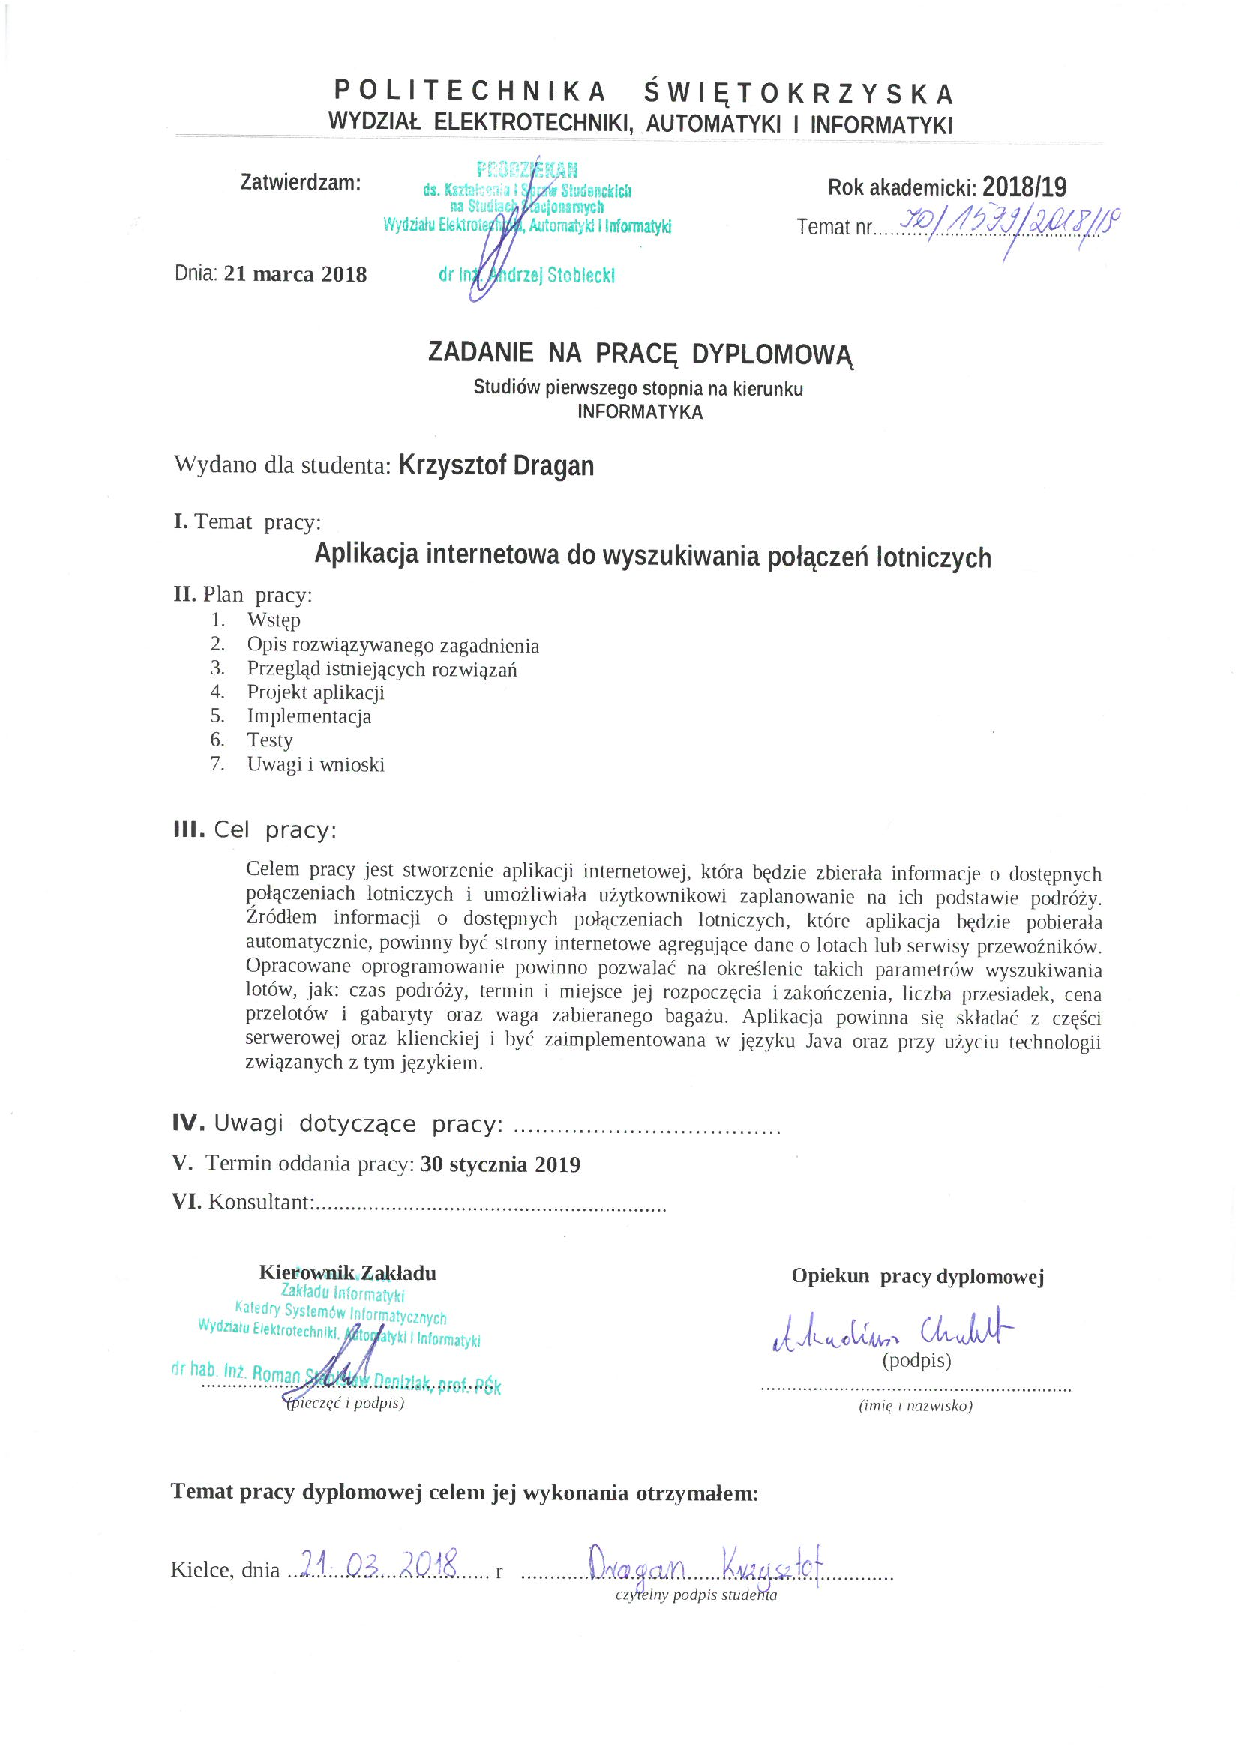
\includepdf[pages=-]{docs/zadanie.pdf}

% --------------------------------------------
% ---------------- Oświadczenie --------------
\afterpage{\blankpage}
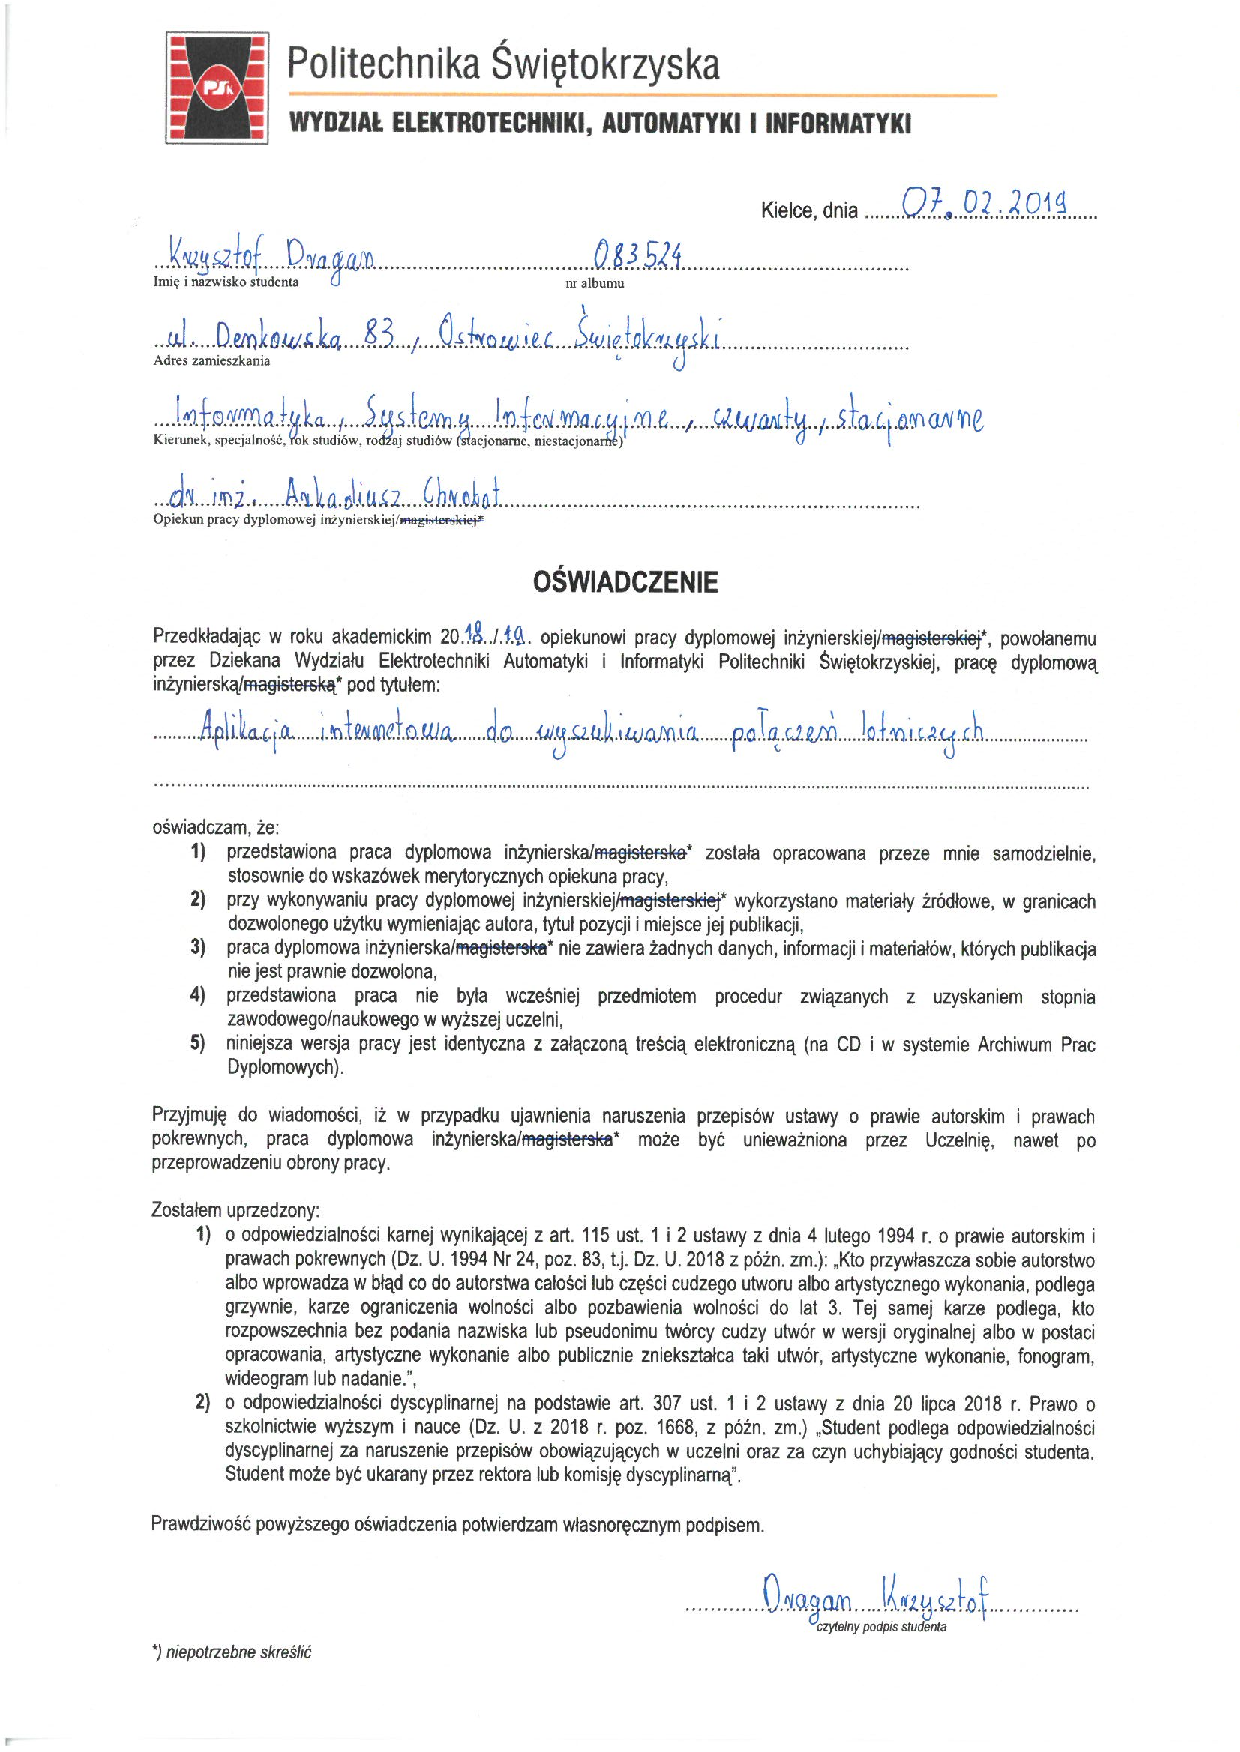
\includepdf[pages=-]{docs/oswiadczenie.pdf}  

% --------------------------------------------
% --------------- Streszczenie ---------------
\thispagestyle{empty}
\begin{center}
	{\fontsize{14pt}{12pt}\selectfont
		\textbf{Aplikacja internetowa do wyszukiwania połączeń lotniczych}}
\end{center}

\begin{flushleft}
	{\fontsize{14pt}{12pt}\selectfont
		\textbf{Streszczenie}}\\
	\vspace{1cm}
\tab Celem niniejszej pracy było stworzenie aplikacji internetowej, która pozwala na wyszukiwanie połączeń lotniczych korzystając z danych zawartych na stronach internetowych przewoźników bądź z innych centr danych. Aplikacja została podzielona na część kliencką oraz serwerową. Klient został napisany przy użyciu technologii Angular 6, natomiast serwer w technologii Java 10. W pracy znajduje się opis architektury stworzonej aplikacji, modułu wyszukiwania połączeń lotniczych a także zagadnień teoretycznych związanych z projektowaniem interfejsu użytkownika dla przeglądarki internetowej.
\end{flushleft}
\vspace{0.5cm}
Słowa kluczowe: Java, Angular 6, REST, programowanie obiektowe, protokół HTTP, programowanie funkcyjne

\vspace{1.5cm}

\begin{center}
	{\fontsize{14pt}{12pt}\selectfont
		\textbf{A web application to search for flight connections}}
\end{center}

\begin{flushleft}
	{\fontsize{14pt}{12pt}\selectfont
		\textbf{Summary}}\\
	\vspace{1cm}
\tab The purpose of the thesis was to build a web application, which will be able to search flight connections using data from websites of airlines or other data sources. The application is splat into two parts: a client and a server. The client was implemented using technology of Angular 6, whereas server in Java 10 technology. Description of architecture built application, module of air connections searching and theoretical issues related to building user interface for web application are included in this thesis. 
\end{flushleft}
\vspace{0.5cm}
Keywords: Java, Angular 6, REST, Object Oriented Programming, HTTP Protocol, Functional Programming
\afterpage{\blankpage}


\renewcommand{\contentsname}{Spis treści}
\pagenumbering{arabic}
\setcounter{page}{9}
\tableofcontents


\chapter*{Wstęp}
\addcontentsline{toc}{chapter}{Wstęp}
Branża lotnicza to jedna z głównych gałęzi współczesnego transportu. Za jej początek uznaje się pierwszy pomyślny lot braci Wright 17 grudnia 1903 roku na polach Kitty Hawk. To wydarzenie zapoczątkowało proces tworzenia się przemysłu lotniczego. W dzisiejszych czasach transport lotniczy uznaje się za najszybszy i najbardziej bezpieczny. Wykorzystuje się go między innymi w transporcie osób, towarów lub też w celach militarnych. Warto wspomnieć też o jego roli w~rozwoju lotów kosmicznych. Dzięki niemu powstała nieosiągalna wcześniej możliwość podróżowania po całym świecie w względnie krótkim czasie.

W ramach niniejszej pracy stworzono aplikację internetową umożliwiającą wyszukiwanie realnych połączeń lotniczych. Aplikacja ta składa się z części klienckiej oraz serwerowej. Celem zwiększenia jej wydajności zastosowano mechanizmy pamięci podręcznej.
Jej głównym zadaniem jest zbieranie danych o połączeniach lotniczych z zewnętrznych serwisów oraz zasobów internetowych. Pozwala ona na uzyskanie informacji o lotach z~uwzględnieniem danych o ich cenie, liniach lotniczych je obsługujących, wymiarach i~wagach dozwolonego bagażu, czasie podróży lub też liczbie przesiadek.

Praca została podzielona na 6 rozdziałów. Rozdział pierwszy przedstawia zagadnienie wyszukiwania połączeń lotniczych wraz z opisem najważniejszych problemów, które starano się rozwiązać w~opracowywanej aplikacji. Drugi rozdział opisuje istniejące rozwiązania w~dziedzinie wyszukiwania połączeń lotniczych, które dostępne są na rynku. Jest to zestawienie dwóch komercyjnych aplikacji które zyskały duże uznanie swoich użytkowników. Rozdział został zakończony podsumowującym porównaniem obu aplikacji. Rozdział trzeci przedstawia projekt aplikacji. Znajdują się w nim schematy z opisem, które przestawiają architekturę powstałej aplikacji. Obrazują one podział funkcjonalności między bazę danych, warstwę logiki biznesowej oraz warstw prezentacji. Opisane zostały również ścieżki komunikacji pomiędzy tymi warstwami.
Rozdział czwarty objaśnia implementację aplikacji. W rozdziale tym zostaną przedstawione najważniejsze fragmenty oprogramowania tworzące funkcjonalność aplikacji. Znajdują się w~nim informacje o użytych technologiach jak i zewnętrznych bibliotekach którymi się posłużono. Piąty rozdział poświęcony jest testom oprogramowania, które potwierdzają zgodne z~wymaganiami działanie aplikacji. Ostatni rozdział przedstawia uwagi i wnioski dotyczące tematu pracy oraz stworzonej aplikacji.

%Poprawić czas przeszły na czas teraźniejszy wg zaleceń doktora
\chapter{Opis zagadnienia}
\label{chp:first}
Głównym zagadnieniem podjętym w pracy jest pozyskanie realnych danych o połączeniach lotniczych  i~zaprezentowanie ich w~kompleksowym interfejsie oraz we względnie krótkim czasie dla użytkownika powstałej aplikacji. Zagadnienie to można podzielić na 3 części:
\begin{itemize}[noitemsep,topsep=0pt]
\item znalezienie źródeł danych o połączeniach lotniczych,
\item parsowanie różnych typów danych,
\item zapewnienie dobrej wydajności podczas wyszukiwania połączeń lotniczych.
\end{itemize}
Części te zostaną opisane w podrozdziałach bieżącego rozdziału.


\section{Źródła danych o połączeniach lotniczych}
Największą trudnością podczas pisania pracy było znalezienie odpowiednich zasobów danych, które nie byłyby płatne oraz zapewniałyby rzetelne i sprawdzone dane lotnicze. Poszukiwania zaczęto od złożenia podań do centrów danych o dostęp do ich zasobów. Większość z nich wymaga opłaty za swoje usługi, które sięgają nawet 10 000\$. Niektóre z nich oferują jednak darmowy, choć limitowany, dostęp. Na potrzeby pracy wybrano serwis FlightLookup jako głównego dostawcę danych. Informacje przez niego dostarczane stanowią większą część odpowiedzi serwera. Darmowy dostęp jest do 500 zapytań w trakcie miesiąca.
Dodatkowymi źródłami danych są:
\begin{itemize}[noitemsep,topsep=0pt]
\item Skyscanner - serwis udostępniający średnie ceny przelotów w określonym przedziale czasowym oraz informacje dotyczące dozwolonego bagażu,
\item Aviation Edge - usługa chmurowa udostępniająca dane o liniach lotniczych,
\item ourairports.com - strona internetowa umożliwiająca pobranie danych o większości lotnisk na świecie.
\end{itemize}
Skyscanner jest komercyjną aplikacją zbierającą wiele rodzajów danych lotniczych. Jej szczegółowe działanie zostanie opisane w następnym rozdziale. W tej części pracy zostanie przedstawione użycie zasobów tego produktu w~stworzonym oprogramowaniu. Zasoby Skyscanner'a dostarczyły danych dotyczących dozwolonego bagażu podczas podróży. Aktualne ceny lotów zostały pobrane z serwisu RapidApi korzystającego wewnętrznie z zasobów aplikacji Skyscanner. Jest on dostępny pod adresem sieciowym: \url{https://rapidapi.com/skyscanner/api/skyscanner-flight-search}.

Użycie jego usług wymaga podania miejsca jak i daty wylotu oraz przylotu. Dodatkowym obowiązkowym parametrem jest unikalny kod walutowy który umożliwiał zwrócenie poprawnych wyników. Oprócz cen przelotów Skyscanner posiada też stronę internetową z tabelą opisującą dozwolone wymiary oraz wagę bagażu podczas przelotu. Adres tej strony to:\\ \url{www.skyscanner.net/news/tips/check-in-luggage-size-and-weight-restrictions}\\
Zawartość tej strony jest parsowana przez część serwerową, jednak to zagadnienie zostanie opisane bardziej szczegółowo w następnym podrozdziale.

Kolejnym ważnym źródłem danych jest usługa chmurowa Aviation Edge. Serwis ten udostępnia dane o liniach lotniczych wykorzystując do tego interfejs REST\footnote{Representational State Transfer}. Do użycia tej usługi wymagane jest podanie unikalnego kodu linii lotniczej w celu jej zidentyfikowania oraz pobrania danych w postaci JSON. Aviation Edge jest bezpłatnym serwisem. Do korzystania z jego zasobów wymagane jest tylko założenie konta w celu uzyskania klucza identyfikującego użytkownika.

Ostatnim źródłem danych jest strona internetowa \textit{ourairport.com} znajdująca się pod adresem internetowm: \url{http://ourairports.com/}. Jej zasobem, który został wykorzystany jako źródło danych jest plik CSV zawierający ponad 50000 rekordów dotyczących lotnisk. Przechowuje on dane z szerokiego spektrum typów lotnisk począwszy od tych małych dedykowanych dla awionetek, aż po największe lotniska świata takie jak London Heathrow Airport. Dane te gromadzone są w pliku CSV, który jest pobierany przez część serwerową. Następnie informacje te są filtrowane w celu wyeliminowania lotnisk obsługujących poniżej 4 tysięcy pasażerów rocznie.

\section{Parsowanie danych}
Dane dostarczane przez zewnętrzne usługi są w różnych formatach. Aby zebrać pełną odpowiedź serwera należy  sparsować pojedyncze elementy a następnie zbudować z nich obiekty języka Java.
\subsection{Język znaczników XML}
XML\footnote{eXtensible Markup Language} to standard formatowania treści wspierany przez organizację W3C. Określa on uniwersalną składnię, używaną przy oznaczaniu danych za pomocą znaczników. Ponadto oferuje standardowy format dokumentów komputerowych. Format ten można dostosowywać do dziedzin tak odmiennych jak witryny WWW, grafika wektorowa, serializacja obiektów, wymiana danych elektronicznych czy systemy poczty głosowej. Oznakowanie XML jest udokumentowane za pomocą specjalnych znaczników. Są to konstrukcje z ogranicznikami w nawiasach trójkątnych. Specyfikacja XML określa, jakie wymagania składniowe musi spełniać takie oznaczenie: w jaki sposób elementy są rozpoznawane przez parsery, jak przedstawiony jest znacznik, jakie nazwy elementów są akceptowalne oraz gdzie elementy powinny być rozmieszczone. Dokumenty słownika XML są podobne do dokumentów HTML\footnote{Hypertext Markup Language}, jednak istnieją pomiędzy nimi zasadnicze różnice. Kluczową różnicą między XML a HTML jest to, że XML umożliwia tworzenie własnych znaczników, podczas gdy w HTML nie ma takiej możliwości\cite{xml}.

\begin{lstlisting}[language=XML, caption=Fragment danych w formacie XML, label=list::xml]
    <FlightDetails TotalFlightTime="PT3H35M"
                   TotalMiles="931"
                   TotalTripTime="PT4H25M"
                   FLSDepartureDateTime="2018-11-15T06:40:00"
                   FLSDepartureTimeOffset="+0100"
                   FLSDepartureCode="WAW"
                   FLSDepartureName="Warsaw"
                   FLSArrivalDateTime="2018-11-15T10:05:00"
                   FLSArrivalTimeOffset="+0000"
                   FLSArrivalCode="LHR"
                   FLSArrivalName="London Heathrow"
                   FLSFlightType="Connect"
                   FLSFlightLegs="2"
                   FLSFlightDays="...4..."
    >
\end{lstlisting}

XML jest językiem znaczników, nie jest on językiem programowania, magazynem danych czy też protokołem transportu sieciowego. XML oferuje możliwość formatowania danych. Zapewnia to im dostępność na wielu platformach i odporność na upływ czasu. W~starszych wersjach standardu XML dokument zapisany za pomocą dowolnego oprogramowania na jednej platformie nie dawał się odczytywać na innej. Wersja 3.2 usunęła tę wadę. Zapewnia ona obsługę Unicode, co oznacza, że dokumenty XML składają się w całości ze znaków należących do zestawu Unicode. 

Wyszukiwanie informacji o połączeniach lotniczych rozpoczyna się od odebrania danych z serwisu FlightLookup w postaci XML. Jest to najważniejsza operacja podczas wyszukiwania połączeń lotniczych. Dane zebrane na tym etapie są parametrami wyszukiwania podczas korzystania ze źródeł danych wykorzystanych w późniejszej fazie tego procesu. Przykład odebranej treści znajduje się na listingu \ref{list::xml}.

Operacja parsowania obiektów XML na obiekty języka Java zostanie dokładniej opisana w rozdziale o implementacji. Załączony listing \ref{list::xml} przedstawia jeden z elementów danych XML o nazwie \textit{FlightDetails}. Zawiera on przykładowe pola takie jak: \textit{TotalMiles} i \textit{FLSFlightDays}. Elementy te zostały odwzorowane w postaci klas języka Java o takich samych nazwach jak nazwa elementu. Powstała klasa posiada też takie same pola jak obiekt w XML.

\subsection{Notacja JSON}
Notacja JSON\footnote{JavaScript Object Notation} jest nowoczesnym sposobem prezentacji danych. Wywodzi się ona z języka JavaScript, w~którym została głównym formatem prezentacji obiektów tej technologii. Notacja JSON jest zbudowana na dwóch strukturach:
\begin{itemize}[noitemsep,topsep=0pt]
\item kolekcji par nazwa/wartość, w zależności od języka programowania zrealizowana jako obiekt, słownik bądź kolekcja danych,
\item uporządkowanej listy wartości, w~większości języków zrealizowanej jako tablica, wektor, lista lub sekwencja.
\end{itemize}
Są to uniwersalne struktury danych. Prawie wszystkie nowoczesne języki programowania wspierają je w odpowiedniej dla siebie formie. Notacja JSON jest to format danych, który jest wymienny między językami programowania. Ta właściwość czyni ją najpopularniejszym formatem wymiany informacji między aplikacjami oraz mikroserwisami\cite{json}. W stworzonej aplikacji dane w tym formacie dotyczyły linii lotniczych oraz cen przelotów. W pierwszym przypadku obiekt JSON można było w prosty sposób skonwertować na obiekt języka Java. Przykładową strukturę zaprezentowano na listingu \ref{list::json}.
Kod źródłowy odpowiedzialny za konwersję tego obiektu zostanie przedstawiony w rozdziale czwartym.
\begin{lstlisting}[language=JSON, caption= Przykładowy obiekt w notacji JSON, label=list::json]
    {
        "airlineId": "1",
        "nameAirline": "American Airlines",
        "codeIataAirline": "AA",
        "iataPrefixAccounting": "1",
        "codeIcaoAirline": "AAL",
        "callsign": "AMERICAN",
        "type": "scheduled",
        "statusAirline": "active",
        "founding": "1934",
        "nameCountry": "United States",
        "codeIso2Country": "US"
    }
\end{lstlisting}

\subsection{Język HTML}
HTML jest standardowym językiem znaczników do tworzenia stron WWW. Dokumenty HTML są podstawową treścią jaką generują przeglądarki internetowe. W pracy dyplomowej źródłem danych o wymiarach i wadze dozwolonych bagaży była strona internetowa aplikacji Skyscanner\cite{html}. Listing \ref{lst::html} przedstawia fragment takich danych zapisanych w formacie HTML.
\begin{lstlisting}[language=HTML5, caption= Fragment dokumentu HTML, label=lst::html]
<table class="tftable" style="height: 3990px" border="1" width="578">
<tbody>
<td><a href="https://www.skyscanner.net/news/tips/aer-lingus-baggage-allowance-explained/">Aer Lingus</a></td>
<td>No free allowance</td>
<td>No size restriction
<p>&nbsp;</p>
<p><strong>32kg</strong> per bag, or<br>40kg across 2 bags</p>
</td>
</tr>
<tr>
\end{lstlisting}

\section{Wydajność wyszukiwania}
Wyszukiwanie tak złożonych danych jak informacje o połączeniach lotniczych, a następnie parsowanie ich, niesie za sobą pewne konsekwencje. Są one związane z~czasem. Użytkownik powinien otrzymać interesującą go treść w jak najkrótszym czasie. W celu poprawy wydajności aplikacji wprowadzono mechanizmy skracające czas odpowiedzi serwera.
Dla zbierania danych dotyczących lotnisk oraz bagażów zaimplementowano rozwiązania polegające na pobieraniu pełnych zbiorów tych informacji do bazy danych lub do pliku tekstowego znajdującego się na serwerze. Pozwoliło to na ograniczenie częstości pobierania danych ze stron lub zewnętrznych baz danych.

Kolejnym rozwiązaniem było wprowadzenie funkcyjnego stylu programowania w kluczowych elementach części serwerowej, które odpowiadały za wyszukiwanie połączeń lotniczych.  Programowanie funkcyjne wprowadzone w Javie 8 pozwala skrócić czas trwania niektórych operacji wykonywanych przez maszynę wirtualną Javy, a więc też czas wyszukiwania lotów.
Implementacje tych rozwiązań są opisane w rozdziale czwartym.

Ostatnim zastosowanym mechanizmem są pamięci podręczne (ang. \emph{cache}) danych. Część danych, która jest gromadzona przez aplikację w~zasobach o długich czasach dostępu i względnie niskiej przepustowości jest dodatkowo przechowywana w pamięci RAM o lepszych parametrach\cite{ehcache}. To rozwiązanie jest często stosowane w~nowoczesnych systemach informatycznych. Odczytywanie danych z tej pamięci jest szybsze w porównaniu na przykład z odczytywaniem dokumentów XML i~JSON z~pamięci masowej, zewnętrznej bazy danych czy też zasobów sieciowych. Przeznaczeniem pamięci masowych jest skracanie czasu odpowiedzi dla określonych zapytań do części serwerowej, które są zwielokrotnione i wykonywane przez wielu użytkowników. Wykonując operacje wyszukiwania lotów, moduł wyszukiwania sprawdza czy w  ~pamięci podręcznej znajdują się poszukiwane wyniki. Jeśli tak, zwraca je użytkownikowi. W przeciwnym wypadku  wyszukuje loty standardowym sposobem a wynik zapisuje do pamięci podręcznej. Dla danych o liniach lotniczych, bagażach oraz dla całego obiektu lotu w części serwerowej stworzono 3 kontenery pamięci podręcznych. Czas przetrzymywania danych w tych kontenerach wynosi odpowiednio: 7 dni, 7 dni oraz 2 godziny. Definiując czasy dla informacji o lotniskach oraz bagażach sugerowano się częstotliwością aktualizowania tych danych przez dostawców. Na ich stronach zmiany są dokonywane średnio raz na kwartał. Ponadto, opracowany serwer zawiera oprogramowanie, które codziennie sprawdza czy nastąpiła jakaś zmiana we wspomnianych zasobach. Jeśli taka sytuacja by wystąpiła, odpowiednie kontenery pamięci podręcznej zostaną wyczyszczone. Dane o połączeniach lotniczych charakteryzują się znacznie większą wrażliwością na zmiany w czasie rzeczywistym. Parametry lotu takie jak data wylotu bądź czas przelotu mogą okazać się dla użytkownika kluczowe i zadecydować o jego wyborze. Z tego powodu czas przetrzymywania tych danych w pamięci podręcznej został ograniczony do 2 godzin. 
Wybór informacji, które powinny znaleźć się w pamięci podręcznej bazuje na tzw. temperaturze danych. Trzy wymienione wcześniej zasoby są najczęściej wykorzystywane przez serwer, dlatego też zdecydowano się na stworzenie dla nich odpowiednich kontenerów pamięci podręcznej.

\chapter{Przegląd istniejących rozwiązań}
Analiza istniejących rozwiązań, czyli aplikacji wyszukujących połączenia lotnicze pozwoliła sprecyzować wymagania względem budowanego oprogramowania. W Internecie można znaleźć wiele aplikacji o podobnej lub takiej samej dziedzinie zastosowania, jak opracowana aplikacja. W tym rozdziale opisane są najbardziej znane wyszukiwarki lotów dostępnych na rynku. 

\section{Wyszukiwarka lotów Skyscanner}
Pierwszym przykładem jest aplikacja internetowa Skyscanner. To wyszukiwarka lotów, która umożliwia użytkownikom szukanie według ceny i lokalizacji. Oprócz wyszukiwania lotów, Skyscanner oferuje opcje szukania hoteli blisko lotnisk oraz wypożyczania auta w pobliżu lotniska docelowego. Warto wspomnieć o~innej jej usłudze, czyli udostępnianiu danych~o połączeniach lotniczych zewnętrznym firmom i programistom. W~związku z~tym aplikacja Skyscanner była brana pod uwagę, jako potencjalne źródło danych. Jej właściciel jednak wymaga dużych opłat za swoje usługi, w warunkach akademickich niemożliwe było skorzystanie z~nich.
Aplikacja ta jest dostępna w ponad 30 językach oraz używana przez 60 milionów użytkowników miesięcznie\cite{skyscanner}. Skyscanner znajduje się pod adresem sieciowym: 
\url{https://www.skyscanner.net/}.

Opisywana aplikacja oferuje swoim użytkownikom szereg przydatnych funkcji. Korzystające z jej osoby mogą posługiwać się kompleksowym modułem wyszukiwania połączeń lotniczych. W panelu wyboru parametrów lotów można określić lotnisko wylotu, lotnisko docelowe jak i daty lotu. Skyscanner oferuje trzy opcje wyszukiwania lotów: z~lotem powrotnym, lot w jedną stronę oraz podróż wieloetapowa. Dodatkowo użytkownik może określić liczbę osób biorących udział w podróży jak i klasę biletu lotniczego. Interesującą funkcją jest możliwość dodania pobliskich lotnisk do tych wybranych przez użytkownika. Znajduje ona zastosowanie, gdy na przykład aplikacja nie może znaleźć lotów z wybranego lotniska. Następuje wtedy wyszukiwanie lotów z pobliskich lotnisk znajdujących się w~zasięgu o~kształcie koła o~zadanej długości promienia.
Oprócz rozbudowanego interfejsu do wyboru parametrów lotów Skyscanner oferuje bardzo dobrą wydajność podczas wyszukiwania. Loty bezpośrednie wyszukiwane są natychmiastowo. Na loty z zaznaczoną opcją możliwych przesiadek trzeba poczekać zwykle kilka sekund. Interfejs aplikacji Skyscanner jest zaprezentowany na ilustracji \ref{fig:skyscanner_main}.

\begin{figure}[!ht]
\centering
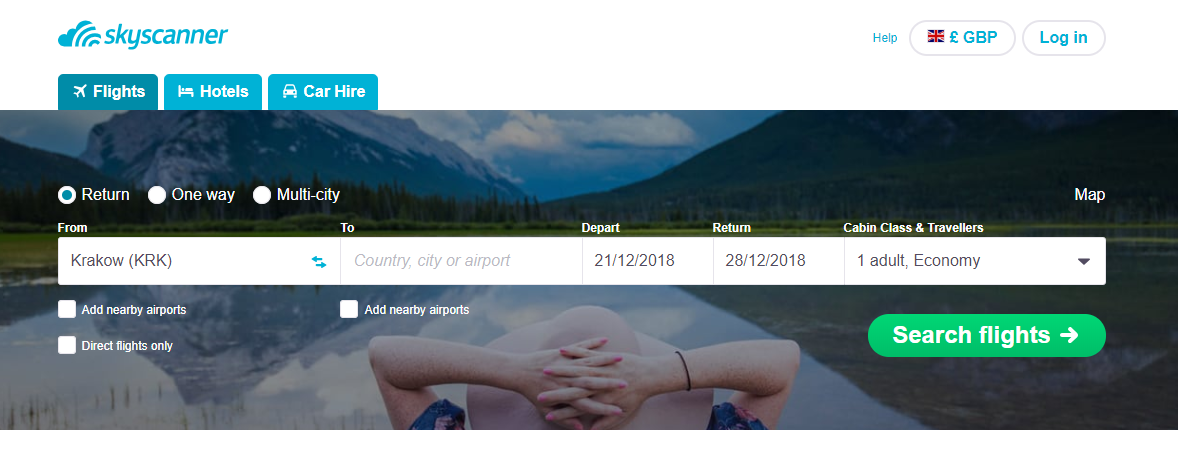
\includegraphics[scale=0.50, keepaspectratio]{skyscanner_main.png}
\caption{Panel wyszukiwania lotów aplikacji Skyscanner}
\label{fig:skyscanner_main}
\end{figure}

Po wybraniu odpowiednich parametrów w~widocznym na rysunku \ref{fig:skyscanner_main} menu należy nacisnąć zielony przycisk po prawej, aby rozpocząć proces wyszukiwania lotów. Przykładowe wyniki zaprezentowano na rysunku \ref{fig:skyscanner_result}. Można na nim zauważyć wyszukane loty z dokładnymi informacjami o linii lotniczej obsługującej lot, miejsca wylotu oraz przylotu, czasie podróży jak i liczbie przesiadek. Z lewej strony dostępny jest panel dzięki któremu można dokonać filtrowania otrzymanych wyników.

\begin{figure}[!ht]
\centering
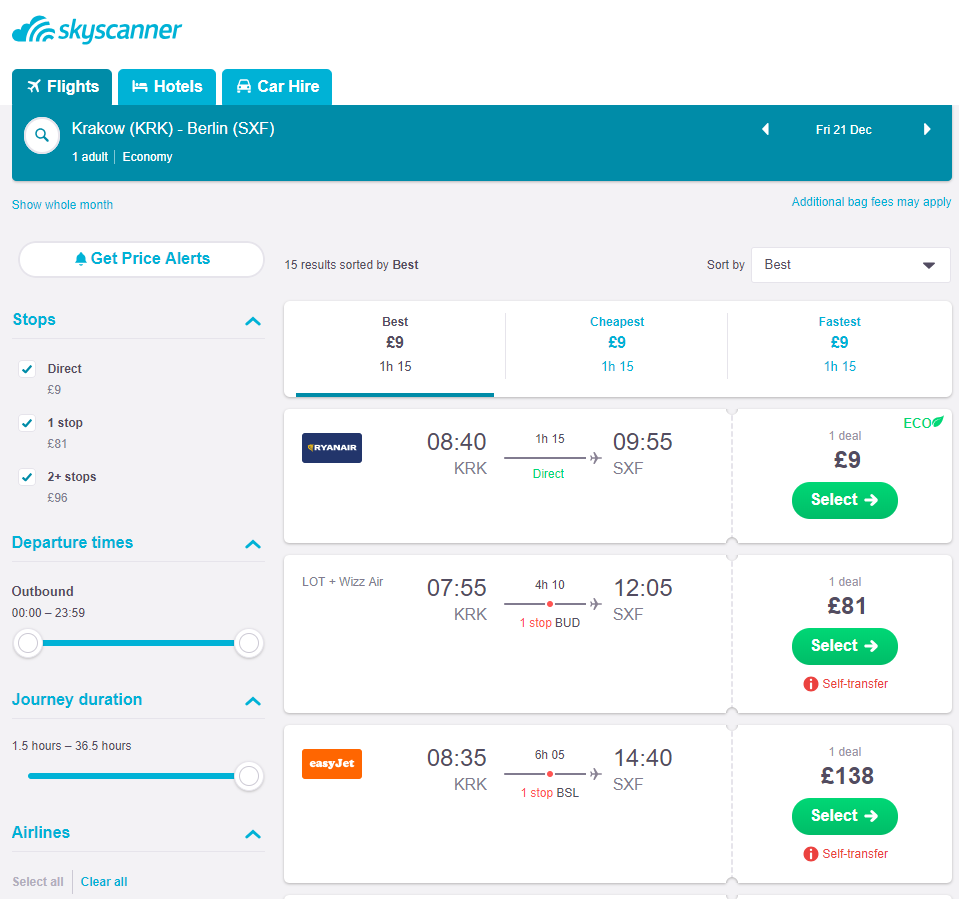
\includegraphics[scale=0.45, keepaspectratio]{skyscanner_result.png}
\caption{Wyniki wyszukiwania lotów aplikacji Skyscanner}
\label{fig:skyscanner_result}
\end{figure}


Warto zwrócić uwagę na panel podróży wieloetapowej, który jest dostępny po kliknięciu  odpowiedniego przycisku powyżej pola wyboru lotniska wylotowego. Można w nim wybrać do siedmiu osobnych połączeń lotniczych i na ich podstawie zaplanować podróż. Każde z tych połączeń jest domyślnie lotem w jedną stronę.
 
\begin{figure}[!ht]
\centering
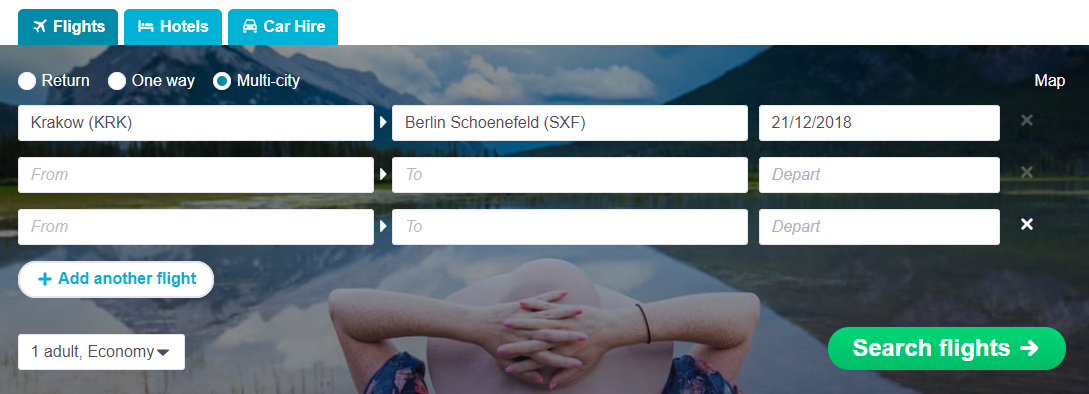
\includegraphics[scale=0.50, keepaspectratio]{skyscanner_multi.png}
\caption{Komponent podróży wieloetapowej}
\label{fig:skyscanner_multi}
\end{figure}

\section{Wyszukiwarka lotów Google Flights}
Kolejnym przedstawianym rozwiązaniem jest aplikacja internetowa Google Flights firmy Google. Jest to jeden z głównych internetowych produktów firmy z Kalifornii, zintegrowany z innymi usługami tej firmy, co czyni go bardzo praktycznym systemem. Google Flights zostało wdrożone 13 października 2011 roku\cite{googleFlights}. Ma zbliżone funkcje do wcześniej opisywanego konkurenta, Skyscanner. Oferuje jednak pewne dodatkowe udogodnienia. Pozwala on użytkownikowi na wyszukiwanie lotów według takich kryteriów, jak czas trwania podróży oraz koszt. Największą zaletą tej aplikacji jest jej efektywność. Silnik tej wyszukiwarki jest podobny do tego stosowanego w~Google Search. Wydajność tego oprogramowania została uzyskana przez użycie wyspecjalizowanych algorytmów szukających firmy Google oraz specjalnemu indeksowaniu danych. Oprócz tej zalety aplikacja prezentuje również czytelny i dostosowujący się do używanego medium (ang. \emph{responsive}) interfejs, który jest dobrze oceniany przez użytkowników.

\begin{figure}[!ht]
\centering
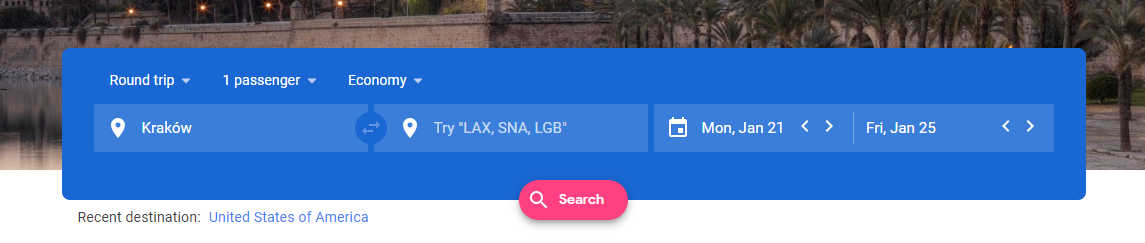
\includegraphics[scale=0.50, keepaspectratio]{google_flights_search_panel.png}
\caption{Panel wyszukiwania lotów aplikacji Google Flights}
\label{fig:google_flights_search_panel}
\end{figure}
Rysunek \ref{fig:google_flights_search_panel} przedstawia panel wyszukiwania lotów oferowany przez opisywaną aplikację. Dostępny jest też komponent podróży wieloetapowej który znalazł się też w poprzednio opisywanej aplikacji oraz w~aplikacji powstałej w~ramach tej pracy.

\begin{figure}[!ht]
\centering
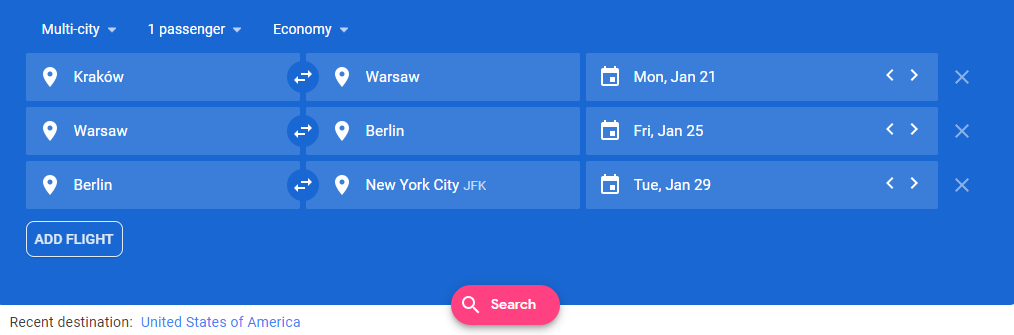
\includegraphics[scale=0.60, keepaspectratio]{google_flights_multi.png}
\caption{Komponent podróży wieloetapowej aplikacji Google Flights}
\label{fig:google_flights_multi}
\end{figure}
Wszystkie produkty firmy Google, które dostępne są za pomocą przeglądarki WWW charakteryzują się specyficznym stylem interfejsu. Jest to styl Material Design, który określa specyfikację pojedynczych elementów aplikacji Google'a. Rysunek \ref{fig:google_flights_result} przedstawia przykładowe wyniki wyszukiwania lotów. Znajdują się one na rozwijanej liście. Po kliknięciu w wybrany element listy rozwija się panel z dokładniejszymi informacjami o locie. Każdy element zaprezentowany na wspomnianym rysunku jest zgodny z Material Design. Widać na przykład zaokrąglenia przycisków charakterystyczne dla produktów marki Google. 

\begin{figure}[!ht]
\centering
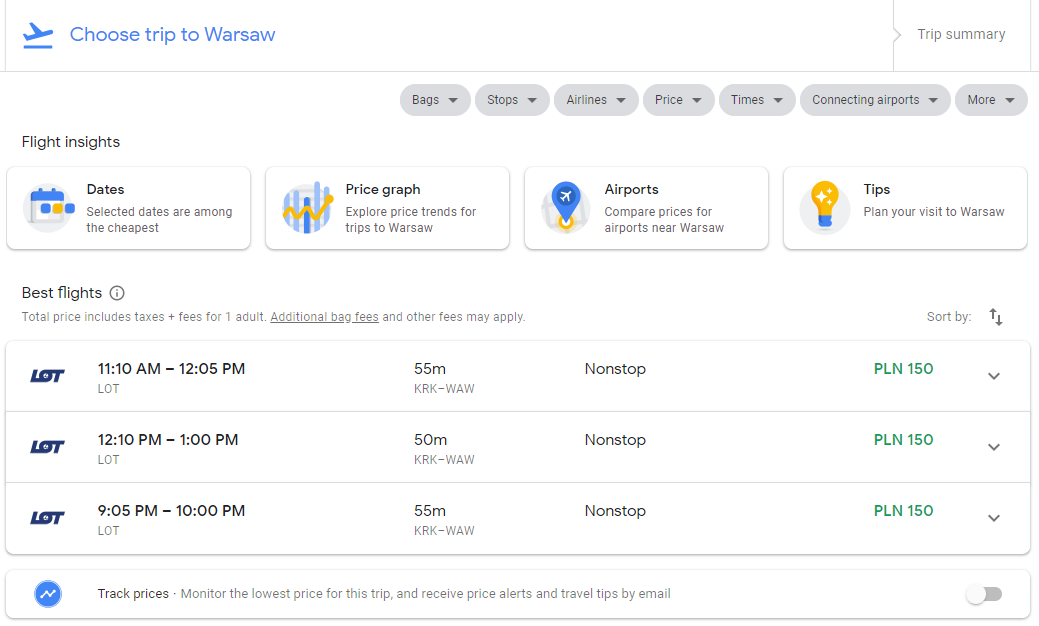
\includegraphics[scale=0.50, keepaspectratio]{google_flights_result.png}
\caption{Wyniki wyszukiwania lotów}
\label{fig:google_flights_result}
\end{figure}


\section{Porównanie aplikacji}
Obie opisane aplikacje są rozwiązaniami komercyjnymi, stworzonymi przez wieloosobowe zespoły programistów. Są także systemami sprawnie działającymi, z czytelnym interfejsem graficznym. Dostarczają one niemal identycznych usług {\dywiz} posiadają tę samą ofertę dla użytkownika, jednak różnią się jakością jej wykonania. 

Zaletą aplikacji Skyscanner jest z pewnością rzetelność jej danych, która jest potwierdzona licznymi nagrodami od linii lotniczych. Warto też wspomnieć o jej systemie wyszukiwania lotów. Liczba wyszukanych lotów z przesiadkami często przekracza sto wystąpień. Świadczy to o zaawansowanym silniku wyszukującym  analizującym różne przypadki połączeń. Za wady można uznać dosyć prosty i niedostosowany do potrzeb urządzeń mobilnych interfejs użytkownika. Nie reprezentuje on poziomu nowoczesnych aplikacji. 

Druga wyszukiwarka jest dopracowanym produktem firmy Google. Wyszukuje ona loty bardziej efektywnie niż rozwiązania konkurencji, między innymi Skyscanner. Google Flights współpracuje z systemami sprzedażowymi większości przewoźników lotniczych. Daje to możliwość kupna biletu bezpośrednio z jej strony WWW bez konieczności przechodzenia na zewnętrzną stronę linii lotniczej. Zaletą wyszukiwarki z pewnością jest dopracowany interfejs zgodny ze standardami firmy Google. Gwarantuje on dostosowanie do używanego medium oraz czytelność prezentowanych danych. Wyszukiwarka Google Flights wydaje się być lepszym rozwiązaniem od aplikacji Skyscanner jednak różnica jakości je dzieląca nie jest duża.

\chapter{Projekt aplikacji}
W tym rozdziale jest opisany projekt aplikacji. Zrozumienie podejmowanego zagadnienia w pracy oraz przegląd istniejących rozwiązań pozwolił określić sposoby realizacji wymaganych funkcji w stworzonej aplikacji.  Kluczową sprawą było też ustalenie odbiorców aplikacji oraz przebiegu procesu wyszukiwania połączeń lotniczych. W tym celu stworzono diagramy aktywności oraz przypadków użycia. Poświęcono osobne podrozdziały dla architektury aplikacji, projektu jej interfejsu użytkownika oraz modułowi wyszukiwania lotów. Na końcu rozdziału znajduje część podsumowująca opracowane rozwiązania i diagramy.

\section{Diagram przypadków użycia}
Diagram przypadków użycia przedstawia funkcje systemu wraz z jego otoczeniem. Jest on specjalnym rodzajem bardziej ogólnego zbioru diagramów UML. Na stronie WWW opisującej te diagramy, Michał Wolski przedstawia ich funkcje następująco: \emph{''Diagramy przypadków użycia pozwalają na graficzne zaprezentowanie własności systemu tak, jak są one widziane po stronie użytkownika.''}\cite{uml}.
\begin{figure}[!ht]
\centering
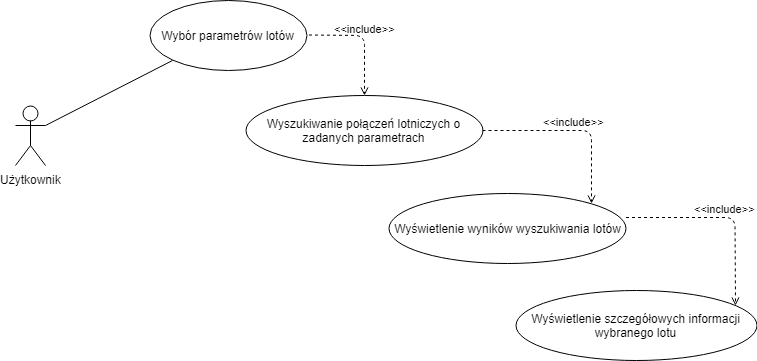
\includegraphics[scale=0.60, keepaspectratio]{usecase_diagram.png}
\caption{Diagram przypadków użycia aplikacji}
\label{fig:usecase_diagram}
\end{figure}

\noindent Zaprezentowany diagram na rysunku \ref{fig:usecase_diagram} obrazuje aktorów i przypadki użycia w stworzonej aplikacji. Uwzględniono w nim tylko jedno aktora, którym jest \textit{Użytkownik}. Reprezentuje on każdą osobę, która korzysta z usług aplikacji. Użytkownik ma możliwość wyboru parametrów lotów, który zawiera się w kolejnym przypadku użycia reprezentującym cały proces wyszukiwania połączeń lotniczych. Jest to oznaczone adnotacją \textit{include}. Kolejnym przypadkiem użycia jest wyświetlenie wyników wyszukiwania lotów. Użytkownik mając te wyniki może wybrać interesujący go przelot i uzyskać o nim dokładniejsze informacje.
\section{Diagram aktywności} 
Diagram aktywności jest diagramem przedstawiającym interakcję dynamicznych aspektów systemu\cite{uml}.

\begin{figure}[!ht]
\centering
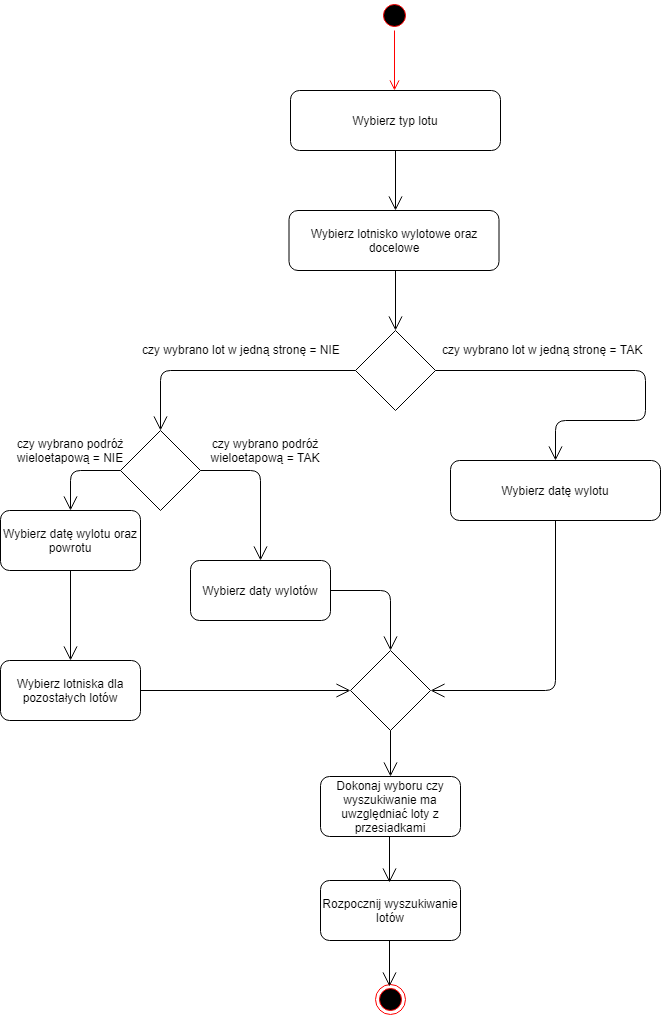
\includegraphics[scale=0.56, keepaspectratio]{activity_diagram.png}
\caption{Diagram aktywności dla procesu wyszukiwania połączeń lotniczych}
\label{fig:activity_diagram}
\end{figure}

Dla opracowanej aplikacji przygotowano diagram aktywności widoczny na rysunku \ref{fig:activity_diagram}. Prezentuje on przebieg kroków, które wykonywane są przez stworzone oprogramowanie. Etap początkowy oraz końcowy został oznaczony czarnym kółkiem. Między nimi znajdują się poszczególne etapy procesu wyszukiwania lotów. Miejsca połączenia różnych ścieżek przebiegu tego procesu lub elementy warunkowe zostały oznaczone rombem.

\section{Architektura aplikacji}
Projektowanie aplikacji rozpoczęto od stworzenia prototypu obrazującego poszczególne części systemu oraz komunikację między nimi. Opracowane oprogramowanie zostało stworzone według architektury trójwarstwowej. Jest ona rodzajem architektury oprogramowania, która składa się z trzech warstw logicznego przetwarzania danych\cite{architektura}.

\begin{figure}[!ht]
\centering
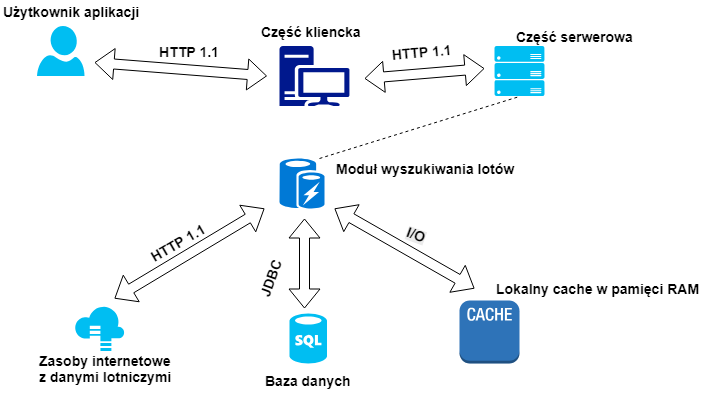
\includegraphics[scale=0.60, keepaspectratio]{architecure_diagram.png}
\caption{Schemat architektury stworzonej aplikacji}
\label{fig:architecure_diagram}
\end{figure}

\noindent Rysunek \ref{fig:architecure_diagram} obrazuje schemat architektury opracowanej aplikacji. Przedstawia on jej trzy warstwy. Pierwszą z nich jest warstwa prezentacji. Renderuje ona treści odpowiednie treści w przeglądarce internetowej. Komunikacja między warstwą prezentacji a logiki biznesowej biznesowej odbywa się z użyciem protokołu HTTP. Warstwa logiki biznesowej obsługuje żądanie tego protokołu przekazując zawarte w nim parametry do modułu wyszukiwania połączeń lotniczych. Z uwagi na jego złożoność zostanie mu poświęcony osobny podrozdział.

\section{Projekt bazy danych}
Baza danych jest używana w~aplikacji jako miejsce dające szybki dostęp do dużego zbioru jakim są dane o lotniskach. Na jej użycie zdecydowano się ze względu na duży rozmiar zasobu informacji reprezentowanych danych oraz sprawdzonych sposobów dostępu do niego.

\begin{figure}[!ht]
\centering
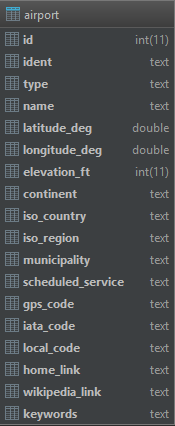
\includegraphics[scale=1.00, keepaspectratio]{database.png}
\caption{Tabela danych lotnisk}
\label{fig:database}
\end{figure}

\noindent Rysunek \ref{fig:database} przedstawia jedyną tabelę znajdującą się w bazie danych, która przechowuje informacje dotyczące lotnisk. Tabela ta zawiera szereg parametrów takich jak na przykład: współrzędne lotniska, jego kody GPS i IATA, nazwę jak i jego typ. Zaprezentowane parametry są określone typami danych w jakich są przechowywane. Dane liczbowe są reprezentowane przez typ całkowity \textit{int} lub przez typ podwójnej precyzji \textit{double}. Parametry oznaczone typem \textit{text} określają ciągi znaków.

%Posprawdzac styl,czy jest opisane tak jak powinno byc dla projektowania
\section{Projekt interfejsu użytkownika}
Klient aplikacji został wyposażony w intuicyjny interfejs użytkownika. Proces jego projektowania polega na tworzeniu schematów lub prototypów. W tym rozdziale zostaną opisane schematy interfejsu użytkownika przygotowane dla strony głównej aplikacji, panelu wyszukiwania lotów oraz dla strony z wynikami wyszukiwania lotów.
\subsection{Projekt strony głównej}
Prototyp strony głównej jest projektem widoku dla strony startowej aplikacji. Na rysunku \ref{fig:main_page_schema} przedstawiono jego schemat.

\begin{figure}[!ht]
\centering
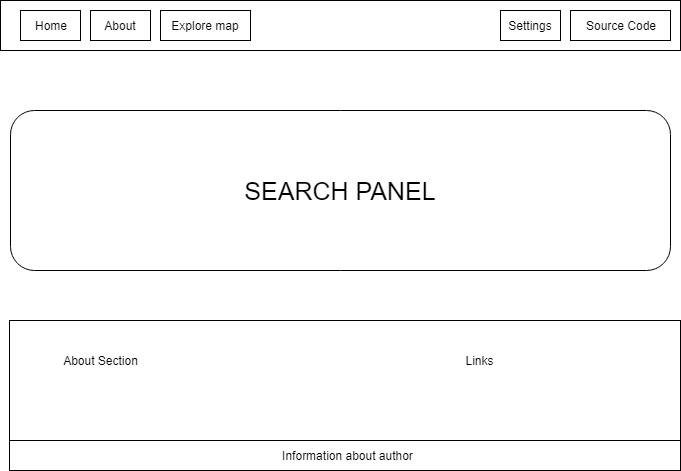
\includegraphics[scale=0.50, keepaspectratio]{main_page_interface_project.PNG}
\caption{Prototyp strony głównej aplikacji}
\label{fig:main_page_schema}
\end{figure}

Górna część strony przedstawia pasek nawigacji, który powinien pozwalać na poruszanie się po aplikacji oraz konfigurujący jej ustawienia. Poniżej zobrazowany jest panel wyszukiwania lotów. Ze względu na jego złożoność został mu poświęcony osobny podrozdział. Dolna część strony ukazuje tak zwaną stopkę. Jest to komponent przeznaczony między innymi do zamieszczenia informacji o autorze aplikacji.
\subsection{Projekt panelu wyszukiwania lotów}
Panel wyszukiwania jest komponentem dynamicznym i podlegającym zmianom pod wpływem wyborów użytkownika. Z tego powodu zaprojektowano dla niego trzy różne widoki. Pierwszy prezentuje panel dla wybranego lotu z możliwością powrotu, drugi obrazuje go dla lotu bezpośredniego, a ostatni przedstawia panel podróży wieloetapowej. Na rysunku \ref{fig:interface_project_departure} zaprezentowano wygląd pierwszego wymienionego panelu.
\begin{figure}[!ht]
\centering
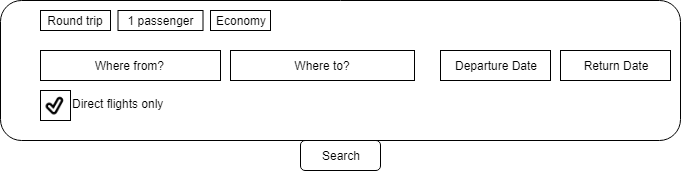
\includegraphics[scale=0.60, keepaspectratio]{interface_project_departure.PNG}
\caption{Prototyp panelu wyszukiwania lotów z możliwością wybrania daty powrotu}
\label{fig:interface_project_departure}
\end{figure}

\noindent W prototypie przewidziano trzy przyciski wyboru typu lotu, liczby pasażerów oraz klasy poszukiwanego biletu. Poniżej zamieszczone są dwa pola do wyboru lotniska wylotowego oraz docelowego. Na prawo od nich znajdują się dwa pola wyboru dat dla wylotu oraz powrotu. 

Dla lotu bezpośrednio wygląd panelu wyszukiwania zmienia się. Zaprezentowano to na rysunku \ref{fig:interface_project_direct} Pole do wyboru daty wylotu powinno być poszerzone , a element wyboru daty powrotu niewidoczny.
\begin{figure}[!ht]
\centering
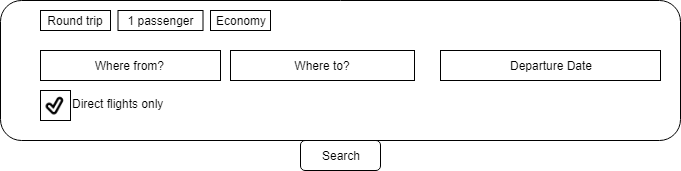
\includegraphics[scale=0.60, keepaspectratio]{interface_project_direct.PNG}
\caption{Prototyp panelu wyszukiwania lotów bezpośrednich}
\label{fig:interface_project_direct}
\end{figure}

Na rysunku \ref{fig:multi_travel_interface} przedstawiono projekt interfejsu dla komponentu podróży wieloetapowej. Można na nim dostrzec dodatkowe przyciski oraz pola.
\begin{figure}[!ht]
\centering
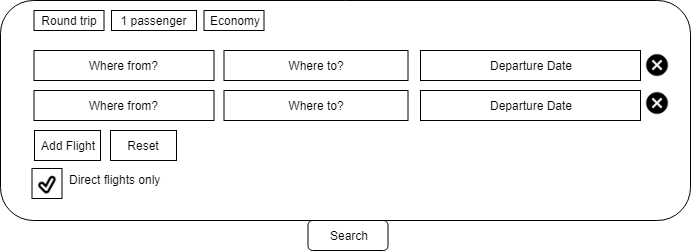
\includegraphics[scale=0.60, keepaspectratio]{multi_travel_interface.PNG}
\caption{Prototyp komponentu podróży wieloetapowej}
\label{fig:multi_travel_interface}
\end{figure}
W komponencie przewidziano elementy wyboru lotnisk i daty wylotu, których liczbę można zwiększać lub zmniejszać odpowiednimi przyciskami. Przycisk oznaczony napisem \textit{Add Flight} dodaje kolejne pola wyboru parametrów lotu. Na prawo od daty wylotu można zauważyć ikonę do usuwania odpowiednich pól. Pozostałe elementy są zaczerpnięte z poprzednio opisanych schematów.
\subsection{Projekt strony z wynikami wyszukiwania}
Ostatnim prototyp dotyczy strony z wynikami wyszukiwania połączeń lotniczych. Zaprezentowano go na rysunku \ref{fig:result_interface} Górna część przedstawia zbiór przewidzianych przycisków, których liczba powinna być zależna od wybranego wcześniej typu lotu. Poniżej zobrazowano listę elementów, które powinny zawierać informacje o wyszukanych lotach. Po kliknięciu w odpowiedni dla elementu listy przycisk powinien rozwinąć się panel z szczegółowymi informacjami o locie.

\begin{figure}[!ht]
\centering
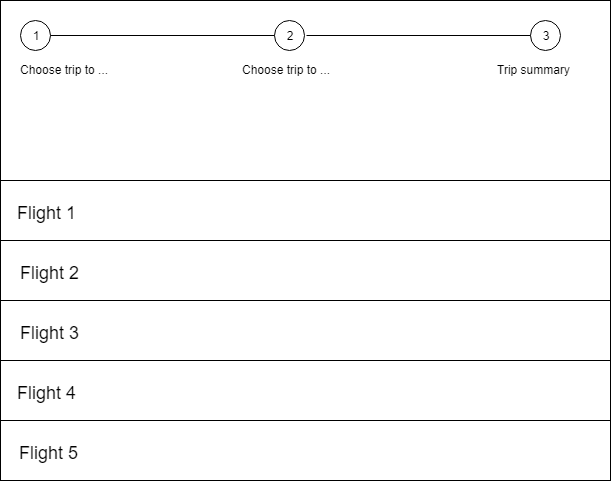
\includegraphics[scale=0.60, keepaspectratio]{result_interface.PNG}
\caption{Projekt strony zawierającej wyszukane loty}
\label{fig:result_interface}
\end{figure}
\section{Moduł wyszukiwania połączeń lotniczych}
Rozwiązanie problemu wyszukiwania połączeń lotniczych jest zadaniem złożonym. Wymaga poradzenia sobie z problemem przeszukiwania wielu źródeł danych oraz konwertowania informacji przez nie zwracanych do postaci, w~której mogą być przetwarzane zarówno przez stronę kliencką, jak i~serwerową. W~związku z~tym wyodrębniono w~strukturze aplikacji moduł, będący elementem części serwerowej oprogramowania, który jest odpowiedzialny za te czynności.

\begin{figure}[!ht]
\centering
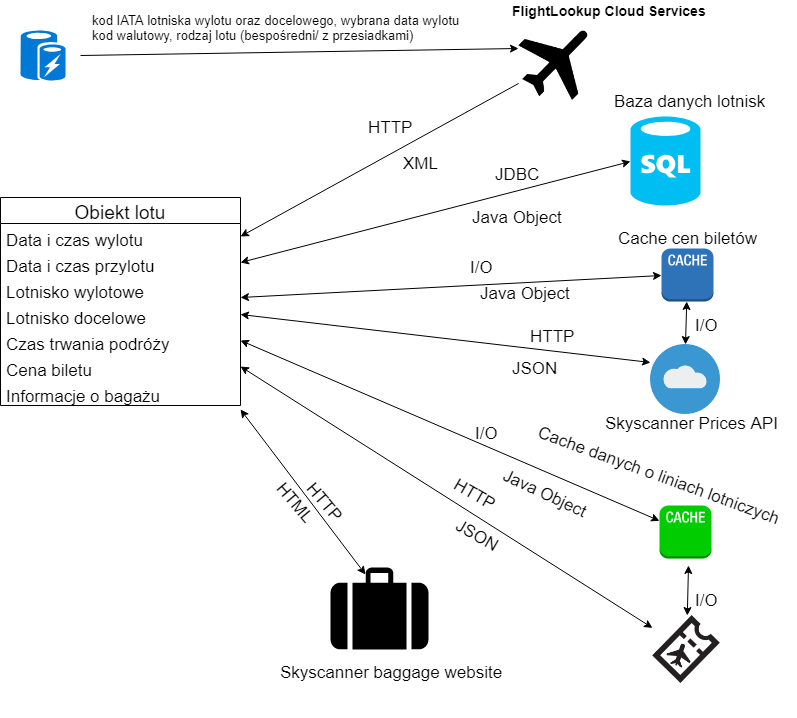
\includegraphics[scale=0.50, keepaspectratio]{search_module.png}
\caption{Schemat architektury modułu wyszukiwania lotów}
\label{fig:search_module}
\end{figure}

Na rysunku \ref{fig:search_module} przedstawiono schemat modułu wyszukiwania połączeń lotniczych wraz ze sposobami pozyskiwania danych do budowy obiektu przez niego zwracanego.
Napisy nad strzałkami są nazwami protokołów służących do realizacji zapytań, a~te pod strzałkami oznaczają format treści zwróconej w~odpowiedzi. Wyszukiwanie zaczyna się od wysłania żądania z kontrolera serwerowego do opisywanego modułu. Żądanie to musi uwzględniać  parametry wyszukiwania. Moduł swoją pracę rozpoczyna od pozyskania danych lotniczych z serwisu FlightLookup. Treść odpowiedzi stanowi większą część całego obiektu lotu, który jest zwracany. Po otrzymaniu tych danych moduł zwraca się do lokalnej bazy danych o udostępnienie informacji dotyczących lotniska na podstawie ich unikalnych kodów IATA\footnote{International Air Transport Association}. Następnym krokiem jest pozyskanie ceny lotu. Czynność ta rozpoczyna się od sprawdzenia, czy poszukiwana informacja znajduje się w pamięci podręcznej. Jeśli takie dane są obecne, to pamięć podręczna zwraca odpowiedni zasób. Jeśli natomiast taka informacja nie jest dostępna, moduł zwraca się do serwerów firmy Skyscanner o udostępnienie cen za poszukiwany przelot. Analogicznie przebiega pozyskiwanie danych o linii lotniczej obsługującej lot. Ostatnim etapem wyszukiwania jest znalezienie informacji o dozwolonym bagażu podczas lotu. Jest to zrealizowane przez zwrócenie się do strony internetowej aplikacji Skyscanner posiadającej aktualne dane. Jej adres został wspomniany w rozdziale drugim. Po zebraniu wszystkich poszukiwanych informacji oraz sparsowaniu ich, obiekt lotu zwracany jest przez moduł wyszukiwania do kontrolera a następnie do części klienckiej gdzie użytkownik może obejrzeć wyniki całego procesu wyszukiwania.

\section{Komunikacja między komponentami aplikacji}
Opisane we wcześniejszych podrozdziałach komponenty narzucają określony sposób komunikacji między nimi. Każdy z nich zostanie przedstawiony w tym podrozdziale.

\subsection{Protokół HTTP}
Protokół HTTP\footnote{Hypertext Transfer Protocol} to jeden z najczęściej stosowanych  protokołów aplikacji w ~Internecie. Jego oryginalnym zastosowaniem jest przesyłanie treści stron WWW. Jest on również stosowany w~innych celach, np. jako protokół dla aplikacji sprzętowych\cite{http}. Cechą protokołu HTTP jest zapisywanie i odczytywanie reprezentacji danych, co umożliwia budowę systemów niezależnych od przesyłanych informacji. Protokół HTTP znalazł szerokie zastosowanie w stworzonej aplikacji. Wysłania żądania z parametrami wyszukiwania lotów możliwe było dzięki zbudowaniu odpowiedniego polecenia GET opisywanego protokołu. Serwer po obsłużeniu żądania odpowiadał treścią w formacie JSON również wykorzystując ten protokół. Dzięki niemu, możliwe było też pobieranie zasobów ze stron WWW oraz zewnętrznych baz danych.
 
\subsection{JDBC}
JDBC\footnote{Java Database Connectivity} to standardowy, niezależny od bazy danych interfejs do interakcji z dowolnym źródłem danych w~którym informacje przechowywane są w~tabelach. Przeważnie jest używany do współdziałania z relacyjnym systemem zarządzania bazami danych. Za pomocą tego interfejsu można też korzystać z~innych źródeł danych, jak arkusz csv, plik tekstowy itd. Zazwyczaj używa się go do łączenia z bazą danych, wyszukiwania danych i ich aktualizowania. Umożliwia on także wykonywanie procedur SQL przy użyciu składni niezależnej od bazy danych\cite{jdbc}. W opracowanej aplikacji interfejs JDBC pośredniczył pomiędzy relacyjną bazą danych a częścią serwerową aplikacji.


\subsection{I/O}
Podprogramy realizujące operacje zapisu oraz odczytu są podstawowymi częściami systemów operacyjnych oraz bibliotek języków programowania. Prawie wszystkie programy komputerowe wykonują pewne operacje zapisu/odczytu inaczej zwanymi operacjami wejściowymi i wyjściowymi. W opracowanej aplikacji za wykonywanie tych operacji odpowiada język Java ,który za pośrednictwem systemu operacyjnego korzysta z~zasobów plikowych lub pamięci podręcznej. Operacje I/O dotyczą systemu plików, który jest elementarnym składnikiem każdego systemu operacyjnego. Zarządza on archiwizacją danych oraz ich późniejszym odzyskiwaniem. System plików przetrzymuje dane w plikach, które zaś są przechowywane w katalogach. Dostęp do plików oraz katalogów uzyskuje się przez zdefiniowanie ścieżek dostępu, które lokalizują obiektu systemu plików\cite{i/o}.
Opracowany serwer wykorzystuje opisane operacje do odczytu pamięci podręcznej, plików CSV oraz plików tekstowych. Czynności te wspomagają pracę serwera pozwalając na szybszy dostęp do zasobów danych.

\section{Podsumowanie}
Zaprezentowane w tym rozdziale projekty oraz schematy pozwoliły zrozumieć sposoby działania aplikacji. Diagramy przypadków użycia oraz aktywności dostarczyły informacji o odbiorach aplikacji oraz o możliwościach jakie ona udostępnia. Schemat architektury trójwarstwowej podzielił aplikacją na logiczne części objaśniając ich funkcje. Podrozdział dotyczący bazy danych pozwolił zrozumieć jej zastosowanie w powstałym systemie. Następnie zrealizowanie schematy interfejsu użytkownika przedstawiły ogólny zarys wymagań postawionych przed implementacją części klienckiej. Ze względu na swoją złożoność w kolejnej części tego rozdziału został omówiony moduł wyszukiwania lotów. Zaprezentował logikę stojącą za skomplikowanym procesem wyszukiwania. Ostatni podrozdział przybliżył rodzaje komunikacji między komponentami aplikacji oraz wyjaśnił ich użycie w aplikacji.



\chapter{Implementacja}
Implementacja aplikacji jest szczegółowo opisana w tym rozdziale. Jego treść została stworzona na podstawie projektu aplikacji oraz zagadnień poruszonych w poprzednich rozdziałach. Aplikacja została opracowana według wymagań otrzymanych na podstawie analizy problemu. Jest ona podzielona na dwie logiczne części: stronę serwerową oraz kliencką. 

\section{Oprogramowanie po stronie klienta}
Aplikacja kliencka została zaimplementowana w technologii Angular 6, otwartym framework'u i platformie do tworzenia SPA\footnote{Single Page Application}. Angular został w całości napisany w języku TypeScript, opiekę nad jego rozwojem sprawuje firma Google. Platforma ta umożliwia tworzenie stron internetowych których treść jest dynamicznie zmieniana bez przeładowywania strony. Przynosi to ogromne korzyści w wydajności aplikacji. Całość kodu napisanego w tym framework'u jest kompilowana do języka JavaScript a następnie renderowana w przeglądarce internetowej. 
\subsection{Podział strukturalny}
Aplikacja kliencka została podzielona na cztery pakiety. Pakiet \textit{layout} przechowuje komponenty, które są wielokrotnie używane do budowy stron WWW. Katalog \textit{model} zawiera odpowiedniki klas modelowych z części serwerowej. Kolejnym elementem jest pakiet \textit{pages}. Znajdują się w nim komponenty renderujące kompletne strony internetowe, które są zbudowane z segmentów umieszczonych w katalogu \textit{layout}. Ostatnią częścią aplikacji klienckiej jest pakiet \textit{services}. Zawiera on oprogramowanie odpowiedzialne za komunikowanie się z serwerem. 

\subsection{Moduły pobierania danych}
W części klienckiej zaimplementowano oprogramowanie odbierające dane z części serwerowej. Pierwszy z nich jest odpowiedzialny za połączenie z modułem wyszukiwania po stronie serwera. Zawiera on dane adresu sieciowego serwera udostępniającego zebrane wyniki wyszukiwania połączeń lotniczych.
\begin{lstlisting}[language=JavaScript, caption= Kod źródłowy funkcji pobierającej wyniki z serwera, label=lst:results]
import { Injectable } from '@angular/core';
import { baseUrl } from '../../../environments/environment';
import { HttpClient } from '@angular/common/http';
import { Observable } from 'rxjs';
import { MultiFlight } from 'src/app/model/interfaces/MultiFlight';

@Injectable({
  providedIn: 'root'
})
export class FlightsService {

  getFlightsURL: string = baseUrl + 'api/flights/';

  constructor(private http: HttpClient) {
  }

  getFlights(originAirport: string, destinationAirport: string, departureDate: string, typeOfConnection: string, currency: string) : Observable<MultiFlight[]>{
    var requestUrl = this.getFlightsURL + originAirport + '/' + destinationAirport + '/' + departureDate + '/' + typeOfConnection + '/' + currency;
    return this.http.get<MultiFlight[]>(requestUrl);   
  }

}
\end{lstlisting}
Na listingu \ref{lst:results} przedstawiono fragment kodu pobierający wyniki wyszukiwania. Funkcja \textit{getFlights} przyjmuje pięć argumentów, które dostarcza jej użytkownik. Pierwszą czynnością tej funkcji jest zbudowanie adresu URL, który posłuży jej do skonstruowania żądania pobrania danych. Jej działanie polega na złączeniu wcześniej wspomnianych parametrów i~stworzeniu żądania GET protokołu HTTP.

Drugim zaimplementowanym serwisem jest prosta funkcja pobierające dane o lotniskach. Jej kod jest przedstawiony na listingu \ref{lst:getAirportsData}
\begin{lstlisting}[language=JavaScript, caption= Kod źródłowy funkcji pobierającej dane lotnisk, label=lst:getAirportsData]
import { Injectable } from '@angular/core';
import { HttpClient, HttpErrorResponse } from '@angular/common/http';
import { baseUrl } from '../../../environments/environment';
import { Airport } from '../../model/interfaces/Airport';
import { Observable, throwError } from 'rxjs';
import { catchError, retry } from 'rxjs/operators';

@Injectable({
  providedIn: 'root'
})
export class AirportsService {

  getAirportsUsingIncompletePhraseURL: string = baseUrl + 'api/airports/getAirportsStartingWith/';

  getAirportsStartingWithPhrase(phrase: string): Observable<Airport[]>{
    return this.http.get<Airport[]>(this.getAirportsUsingIncompletePhraseURL + phrase).pipe(catchError(this.handleError)); 
  }  
}
\end{lstlisting}
Działanie przedstawionego kodu źródłowego rozpoczyna się od stworzenia adresu URL pod którym część serwerowa udostępnia poszukiwane dane. Do zmiennej \textit{baseUrl} oznaczającej domenę serwera zostaje dodana część sparametryzowana dla danych o lotniskach. Funkcja zwraca obiekty typu \textit{Airport} oraz dodatkowo obsługuje błędy zwrócone z drugiej części aplikacji.

\subsection{Interfejs graficzny}
Walory efektywności oraz użyteczności aplikacji tracą na znaczeniu jeśli budowane oprogramowanie nie jest wyposażone w czytelny interfejs użytkownika. Umożliwia on sprawną interakcję pomiędzy użytkownikiem a aplikacją.  Opracowane środowisko graficzne jest grupą wzajemnie współpracujących przycisków oraz obrazów zapewniających nawigację po aplikacji klienckiej w obrębie przeglądarki internetowej. 
W części klienckiej zaimplementowano responsywny wygląd z takimi komponentami jak panel wyszukiwania lotów oraz panel podróży wieloetapowej. Ich kształt i funkcje zostały częściowo zaczerpnięte z rozwiązań rynkowych aby zwiększyć użyteczność aplikacji klienckiej. 
W bieżącym podrozdziale zostanie przedstawiony interfejs aplikacji wraz z krótkim opisem.
\begin{figure}[!ht]
\centering
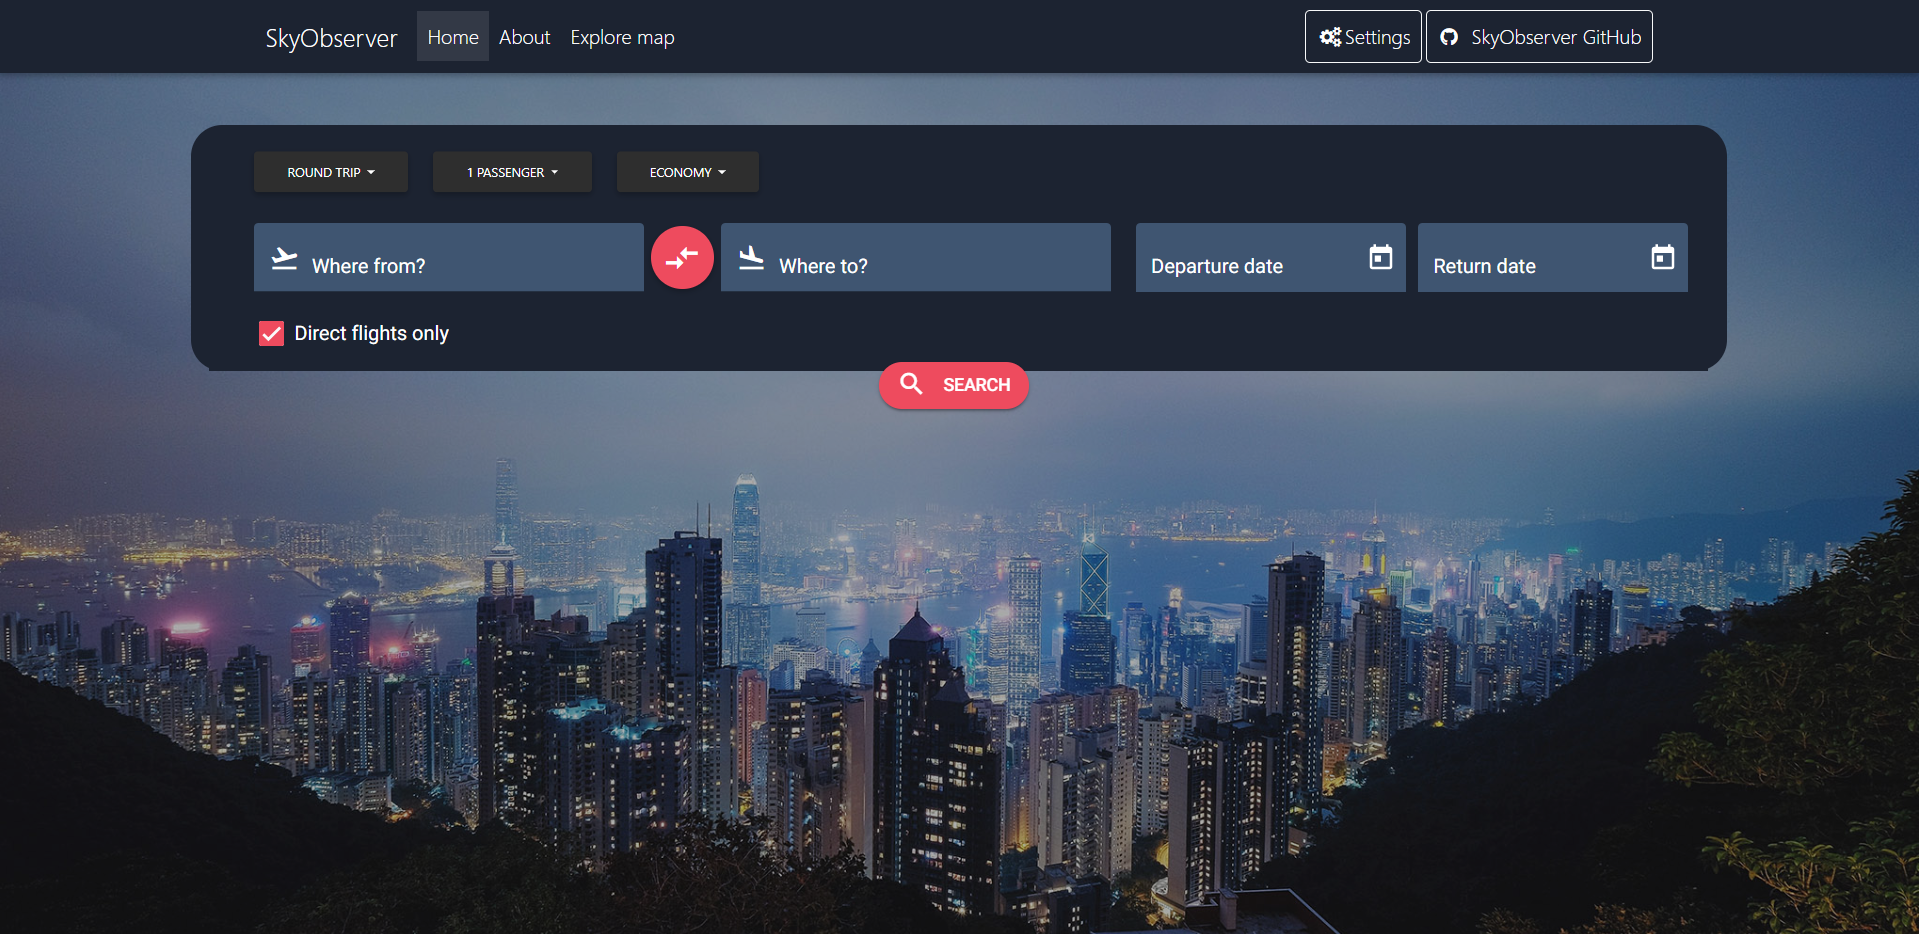
\includegraphics[scale=0.32, keepaspectratio]{client_main_page.png}
\caption{Strona główna aplikacji klienckiej}
\label{fig:client_main_page}
\end{figure}
Rysunek \ref{fig:client_main_page} przedstawia stronę startową części klienckiej. Jego tło jest na całej szerokości oraz długości wypełnione obrazem miasta Hongkong. Górna część strony przedstawia pasek nawigacyjny aplikacji, panel ustawień oraz odwołanie do repozytorium kodu stworzonej pracy dyplomowej. Następnym komponentem aplikacji klienckiej jest panel wyszukiwania lotów.
\begin{figure}[!ht]
\centering
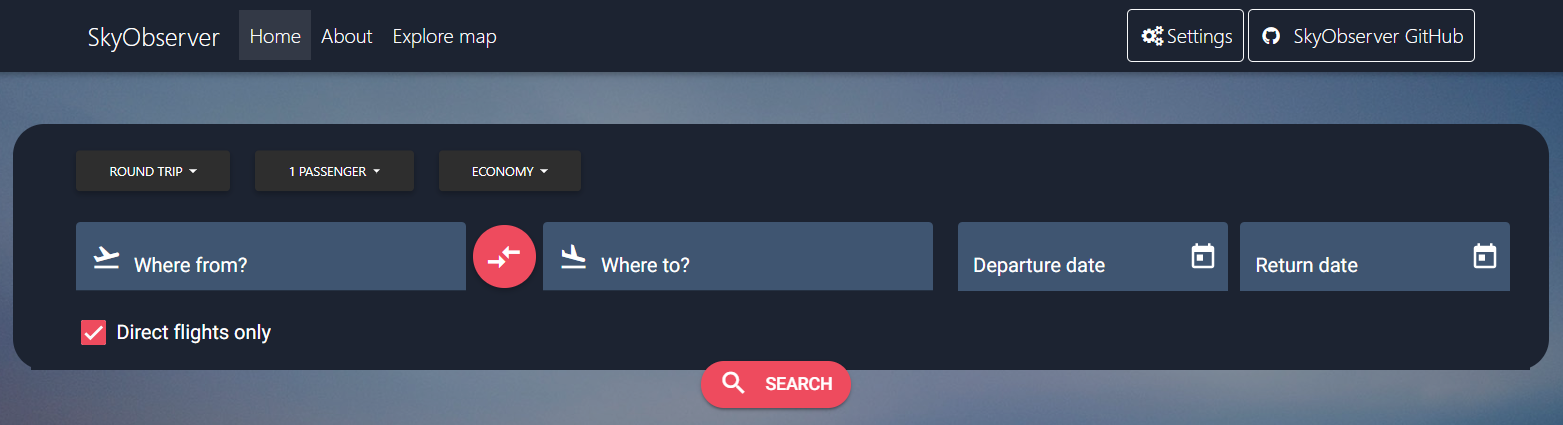
\includegraphics[scale=0.39, keepaspectratio]{search_panel.png}
\caption{Panel wyszukiwania połączeń lotniczych}
\label{fig:search_panel}
\end{figure}
Przedstawiony na rysunku \ref{fig:search_panel} komponent obrazuje rozmieszczenie przycisków, pól wyboru parametrów wyszukiwania oraz dostępne opcje konfiguracyjne. Górna część panelu zawiera trzy przyciski zmieniające ustawienia aplikacji. Odpowiadają one kolejno za wybór rodzaju lotu, liczby pasażerów oraz klasy poszukiwanego biletu lotniczego. W aplikacji założono trzy typy lotów: lot z możliwością powrotu, lot bezpośredni oraz podróż wieloetapową. Kolejna część, poniżej opisanych przycisków przedstawia pola do wyboru parametrów wyszukiwania. Ich liczba zmienia się w zależności od wybranego typu lotu.

W elementach wyboru lotnisk został zaimplementowany mechanizm podpowiedzi wyszukiwania. Użytkownik po wpisaniu kilku pierwszych liter poszukiwanego miasta ma możliwość zobaczyć listę proponowanych lotnisk w obrębie tej miejscowości. 
\begin{figure}[!ht]
\centering
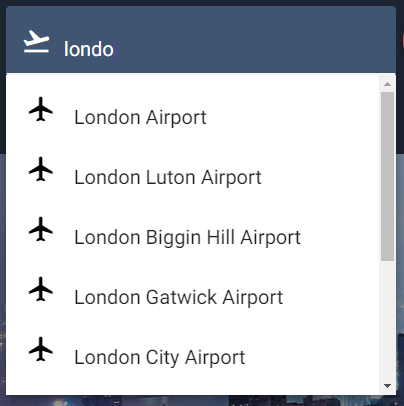
\includegraphics[scale=0.8, keepaspectratio]{airport_choose.png}
\caption{Komponent wyboru lotniska}
\label{fig:airport_choose}
\end{figure}
Operacja ta jest dokonywana poprzez pobranie wpisanych liter a następnie zgłoszenia żądania do części serwerowej, która zwraca wyniki z bazy danych. Implementacja tego mechanizmu jest opisana w poprzednim podrozdziale. Użytkownikowi wyświetlane są pełne nazwy lotnisk. Po wybraniu poszukiwanego miejsca widoczna jest nazwa miasta wraz z unikalnym kodem IATA identyfikującym lotnisko. Efekty wizualne działania tych mechanizmów zostały zaprezentowane na rysunku \ref{fig:airport_choose} Elementem umieszczonym pomiędzy polami dotyczącymi wyboru lotnisk jest przycisk zamiany pól. Jego funkcją jest zamiana informacji zawartych w polach miejsca odlotu oraz przylotu. Ostatnimi elementami są pola wyboru dat lotu docelowego oraz powrotnego. Obecność drugiego jest uzależniona od wybranego typu lotu. W przypadku gdy wyszukiwany jest tylko lot w jedną stronę element ten jest niewidoczny a szerokość pierwszego jest większa. Kliknięcie w ikonę kalendarza wyzwala okno modalne z jego powiększonym widokiem. Szarym okręgiem jest na nim zaznaczony dzień bieżący. Po wybraniu, data zapisywana jest w pamięci aplikacji. Ten zabieg służy przeciwdziałaniu pomyłkom użytkownika przy wyborze daty powrotu. Jeśli taka się pojawi, to aplikacja wskaże zapisaną datę jako najwcześniejszą wartość przy wyborze daty lotu powrotnego. Umożliwia on zaplanowanie podróży złożonej z maksymalnie pięciu lotów w jedną stronę. 
\begin{figure}[!ht]
\centering
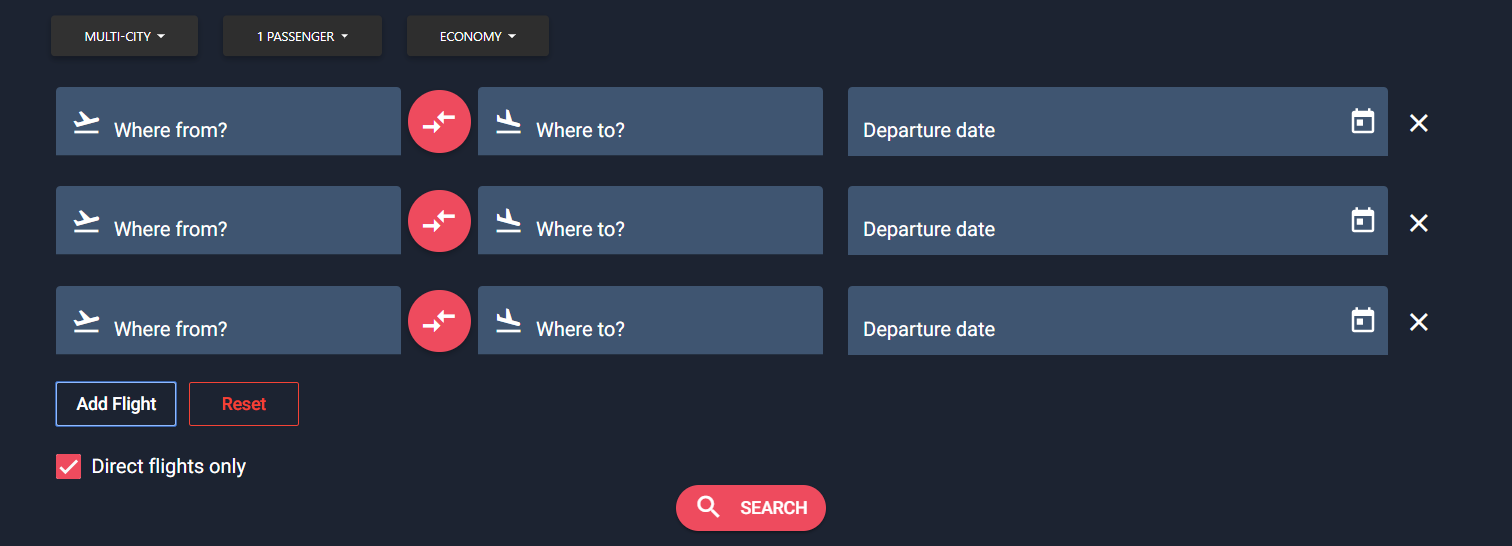
\includegraphics[scale=0.40, keepaspectratio]{multi_panel.png}
\caption{Komponent podróży wieloetapowej}
\label{fig:multi_panel}
\end{figure}
Rysunek \ref{fig:multi_panel} przedstawia wygląd opisywanego komponentu. Interfejs oferuje przyciski do dodawania kolejnych etapów podróży oraz ich usuwania.  

Wspólnym elementem zarówno dla wszystkich modułu podróży jest przycisk wyszukiwania. Po kliknięciu go, aplikacja pobiera wprowadzone przez użytkownika parametry wyszukiwania i przekazuje je dalej do modułu odpytującego serwer. Moduł ten został przedstawiony w poprzednim podrozdziale. Przykładowe wyniki wyszukiwania zaprezentowano na rysunku \ref{fig:result_component} Jest to lista połączeń lotniczych pomiędzy wybranymi miejscami. Każdy element z tej listy jest rozwijalny, co oznacza że po kliknięciu na niego wysunie się dodatkowy obszar ze szczegółowymi informacjami o locie. W zależności od typu lotu wyświetlana jest zmienna liczba komponentów do wyboru połączenia lotniczego na wybranej trasie.
\begin{figure}[!ht]
\centering
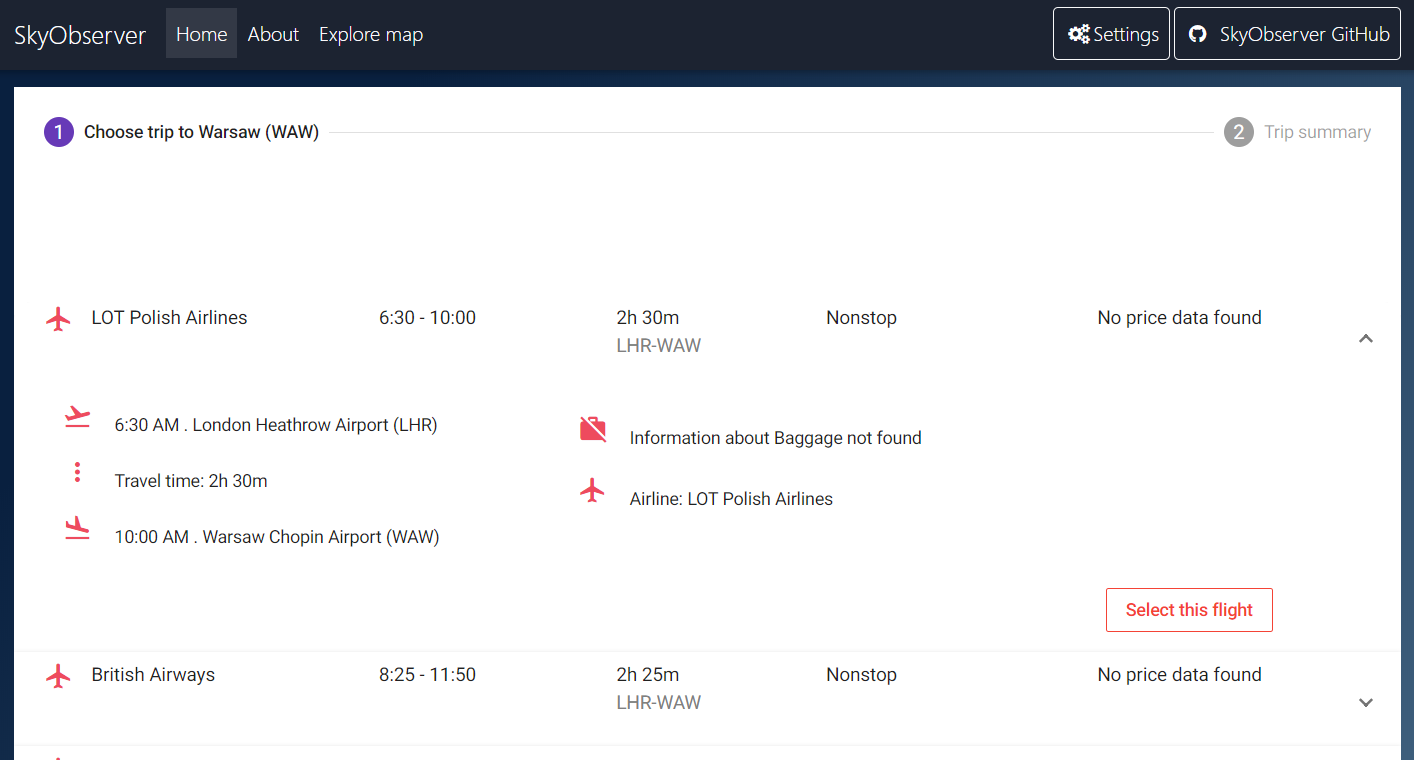
\includegraphics[scale=0.40, keepaspectratio]{result_component.png}
\caption{Wyniki wyszukiwania}
\label{fig:result_component}
\end{figure}

\section{Oprogramowanie po stronie serwera}
Oprogramowanie serwerowe stanowi większą część aplikacji. Zostały w nim zaimplementowane mechanizmy parsowania, wyszukiwania i udostępniania danych lotniczych. W bieżącej części pracy zostanie opisana struktura części serwerowej, oprogramowanie odpowiedzialne za parsowanie różnych rodzajów danych, jak i zaimplementowany moduł wyszukiwania.
Do opracowania aplikacji serwerowej posłużono się językiem programowania Java w wersji 10 oraz pakietami oprogramowania Spring i Hibernate. Java jest językiem programowania z ponad 20 letnią historią. Pierwotnie stworzona i rozwijana przez Jamesa Goslinga została przejęta przez korporację Oracle. Głównym założeniem tego języka jest sentencja \textit{"Napisz raz, uruchom wszędzie"}. Te słowa przemawiają za specjalnym mechanizmem kompilowania i uruchamiania kodu przez Javę. Proces zaczyna się od skompilowania plików o rozszerzeniu java do bytecode'u czyli specjalnej sekwencji bajtów rozumianej przez JVM\footnote{Java Virtual Machine}\cite{jvm}.
Powstałe oprogramowanie serwerowe jest też w dużej mierze oparte na zewnętrznych bibliotekach platformy Spring Framework w wersji 5.
\subsection{Podział na pakiety}
Kod części serwerowej został podzielony na pakiety, których nazwa określa ich rolę w~aplikacji. Ten podział został przedstawiony na rysunku \ref{fig:server_structure}.
\begin{figure}[!ht]
\centering
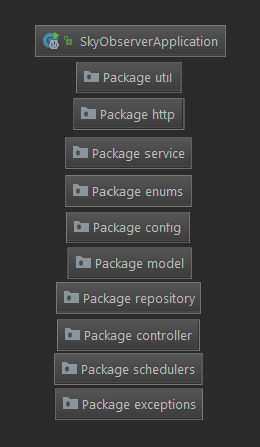
\includegraphics[scale=0.90, keepaspectratio]{server_structure.png}
\caption{Podział strukturalny części serwerowej}
\label{fig:server_structure}
\end{figure}
Zadaniem pakietu \emph{config} jest konfiguracja różnych parametrów serwera podczas jego startu. Ustawia on takie dane jak klucze dostępowe do zasobów lotniczych, parametry pamięci podręcznej oraz zabezpieczenia aplikacji. Warstwa modelowa aplikacji znajduje się w pakiecie \textit{model}. Zaimplementowane zostały w nim klasy modelowe. Są to klasy, które są zwracane przez serwer jako wynik wyszukiwania lotów. Związanym z tym pakietem jest katalog \textit{repository}. Jest on miejscem na klasy implementujące pozyskiwanie obiektów odpowiadających klas modelowych. Niektóre z nich używają swoich odpowiedników z pakietu \textit{service}. Potrzeba ta wynika z konieczności parsowania niektórych formatów danych na obiekty języka Java. Pakietem który udostępnia obiekty modelowe dla części klienckiej jest katalog \textit{controller}. Kod odpowiedzialny za wysyłanie żądań HTTP zaimplementowany jest w części \textit{http}. W części serwerowej zaimplementowano też moduły, które są wywoływane cyklicznie. Aktualizują one lokalne pliki przechowujące dane o lotniskach oraz bagażach. Ich kod jest umieszczony w katalogu \textit{schedulers}. Pozostałe pakiety, czyli \textit{util, enums} oraz \textit{exceptions} zawierają mniej znaczące dla aplikacji funkcje.  

\subsection{Oprogramowanie wyszukujące połączenia lotnicze}
Projekt modułu wyszukiwania połączeń lotniczych został opisany w poprzednim rozdziale, bieżący jest poświęcony kwestiom jego implementacji. Na potrzeby tego modułu opracowano specjalny sposób tworzenia obiektu lotu. Standardowy proces powstawania obiektu związany z~wywołaniem konstruktora okazał się mało przydatny dla wielu obiektów wchodzących w skład jednostki połączenia lotniczego. Do tworzenia tego obiektu zastosowano wzorzec projektowy \textit{Budowniczy}, który opisuje algorytm uzyskiwania złożonego obiektu z innych. Algorytm ten powinien być niezależny od składowych obiektu. Ponadto proces budowania powinien zezwalać na budowę różnych form tworzonego obiektu\cite{builder}.
Klasa modelowa \textit{Flight} została wyposażona w~klasę wewnętrzną budującą jej obiekty. Implementacja tej klasy jest przedstawiona na listingu \ref{lst:attributes}.
\begin{lstlisting}[language=java, caption=Fragment klasy Flight, label=lst:attributes]
public class Flight {
    private String departureTime;
    private String arrivalTime;
    private Airport originAirport;
    private Airport destinationAirport;
    private String duration;
    private CachedPrice price;
    private Airline airline;
    private Baggage baggage;
    
public static class Builder{
     private String departureTime;
     private String arrivalTime;
     private Airport originAirport;
     private Airport destinationAirport;
     private String duration;
     private CachedPrice price;
     private Airline airline;
     private Baggage baggage;
        
     public Flight build(){
           return new Flight(this);
     }   
}
\end{lstlisting}
Klasa odpowiedzialna za zbieranie danych o połączeniach lotniczych jest umieszczona w~pliku \textit{FlightsRepository}. W jej kodzie źródłowym zaimportowano wszystkie pozostałe repozytoria danych. 
Działanie tej klasy polega na zapisaniu w~jej atrybutach, widocznych na listingu \ref{lst:attributes}, wartości pobranych z~odpowiednich repozytoriów. Ze względu na złożoność oraz wielkość implementacji jej kod nie jest umieszczony w~całości w tym rozdziale.

\subsection{Parsowanie danych}
W~tym podrozdziale opisane są implementacje mechanizmów parsowania formatów danych przedstawionych w~rozdziale trzecim. Opracowano następujące klasy parsujące:
\begin{itemize}[noitemsep,topsep=0pt]
\item AirlineParser - parser danych o liniach lotniczych konwertujący obiekty JSON na obiekty Java,
\item AirportsParser - komponent pozyskujące obiekty z plików CSV,
\item BaggagesParser - moduł parsujący dokumenty HTML,
\item PricesParser - klasa konwertująca obiekty JSON zawierające cen lotów,
\item FlightsParser - moduł parsujący złożone dane otrzymane w języku znaczników XML na odpowiadające im obiekty języka Java.
\end{itemize}
Parser linii lotniczych ma najprostszą budowę z~nich wszystkich i~dlatego zostanie przedstawiony jako pierwszy.
\begin{lstlisting}[language=java, caption=Implementacja parsowania treści JSON, label=lst:jsonParsing]
public class AirlineParser {
    private static final int FIRST_ELEMENT = 0;
    private Gson gson = new Gson();

    public Airline getAirlineObjectFromJSONResponse(String jsonObject) {
         Airline[] airlines = gson.fromJson(jsonObject, Airline[].class);
         return airlines[FIRST_ELEMENT];
    }
}
\end{lstlisting}
Listing \ref{lst:jsonParsing} przedstawia kod dokonujący konwersji treści w formacie JSON. Do tego celu posłużono się biblioteką gson firmy Google. Konwersja obiektów JSON na obiekty \emph{Airline} odbywa się poprzez wywołanie metody \emph{fromJson} na obiekcie klasy \emph{Gson}. Funkcja jako wynik zwraca pierwszy element przekonwertowanej tablicy danych.

Translacja treści zwróconej z serwisu \textit{Flight Lookup} otrzymanej w postaci XML odbywa się przy pomocy biblioteki Jackson. Po tej czynności wywoływana jest metoda konwertująca, przedstawiona na listingu \ref{lst:xmlParsing}.
\begin{lstlisting}[language=java, caption=Implementacja parsowania treści XML, label=lst:xmlParsing]
public class FlightsParser {
    private JacksonXmlModule xmlModule = new JacksonXmlModule();

    public OTA_AirDetailsRS getDeserializedXML(String XML) throws IOException {
        xmlModule.setDefaultUseWrapper(false);
        ObjectMapper objectMapper = new XmlMapper(xmlModule);
        return objectMapper.readValue(XML, OTA_AirDetailsRS.class);
    }
}
\end{lstlisting}
Kod klasy FlightsParser jest podobny do poprzedniej przedstawionej na listingu \ref{lst:jsonParsing}. Metoda \textit{getDeserializedXML} jako argument przyjmuje ciąg znaków XML. Do konwersji używana jest klasa \textit{ObjectMapper} pochodząca ze wcześniej wspomnianej biblioteki Jackson. Wynikiem zwróconym przez funkcję jest pojedynczy obiekt \textit{OTAAirDetailsRS} zawierający listę wszystkich wyszukanych lotów.
Ze względu na złożoność kodu źródłowego pozostałych parserów ich implementacja nie zostanie przedstawiona. Kod ten można znaleźć w dołączonym repozytorium, w pakiecie \textit{service}.

\subsection{Zabezpieczenia}
W części serwerowej opracowano zabezpieczenie ograniczające dostęp do udostępnianych danych lotniczych.
\begin{lstlisting}[language=java, caption=Implementacja zabezpieczanie dostępu do serwera, label=lst:security]
@Configuration
@EnableWebMvc
public class CorsConfiguration implements WebMvcConfigurer {

    @Override
    public void addCorsMappings(CorsRegistry registry) {
        registry.addMapping("localhost:4200/**");
    }
}
\end{lstlisting}
Listing \ref{lst:security} przedstawia implementację tego zabezpieczenia. Ustawia ono dostęp do serwera tylko z adresu części serwerowej podanego jako argument metody \textit{addMapping}. Zabieg ten chroni przed dostępem do danych z~niepożądanych adresów sieciowych. 

Mechanizm pamięci podręcznej, usprawniający wydajność aplikacji zminimalizował również szanse na skuteczny atak DDOS. Atak ten uniemożliwia dostęp do usług udostępnianych przez zaatakowane systemy\cite{ddos}. Zabezpieczenie polegające na zastosowaniu pamięci podręcznej zostało krótko opisane w rozdziale pierwszym w, którym przedstawiono trzy kontenery pamięci podręcznej zaimplementowane w aplikacji. Wydajność ich odpowiedzi uodparnia część serwerową na nadmierny ruch sieciowy ze strony użytkowników aplikacji. Zdefiniowano dla każdego z~kontenerów maksymalny rozmiar przechowywanych danych wynoszący 1GB. Po jego przekroczeniu, pamięć podręczna zostaje wyczyszczona.

\subsection{Kontrolery serwera}
W części serwerowej stworzono specjalny komponent odpowiedzialny za obsługę żądań wyszukiwania lotów oraz zwrócenie wyników. 
\begin{lstlisting}[language=java, caption=Kontroler zwracający wyniki wyszukiwania lotów, label=lst:flightsController]
@RestController
@RequestMapping("/flights")
public class FlightsController {

    @Autowired
    private MultiFlightsRepository multiFlightsRepository;

    @GetMapping(value = "/{from}/{to}/{date}/{connection}/{currency}", produces = MediaType.APPLICATION_JSON_VALUE)
    public Collection<MultiFlight> searchForFlights(@PathVariable String from, @PathVariable String to, @PathVariable String date, @PathVariable String connection, @PathVariable String currency) throws AirportsNotFoundException, IOException {
        Collection<MultiFlight> flights = multiFlightsRepository.searchForMultiFlights(from, to, date, connection, currency);
        if (flights.isEmpty()){
            throw new FlightsNotFoundException();
        }
        return flights;
    }
}
\end{lstlisting}
Ten kontroler został zaimplementowany w pakiecie \textit{controller}. Dwie adnotacje nad deklaracją klasy \ref{lst:flightsController} tworzą w serwerze specjalne miejsce, w którym po podaniu odpowiednich parametrów kontroler zostanie wywołany. Parametry te opisane są nad deklaracją metody \textit{searchForFlights}. Funkcja pobiera z adresu URL kody IATA lotniska wylotowego oraz docelowego, datę wylotu, typ połączenia i kod walutowy. Przedstawione parametry są przekazywane metodzie \textit{searchForMultiFlights} z klasy \textit{MultiFlightsRepository}, która zwraca wyniki wyszukiwania w postaci kolekcji obiektów. W przypadku nie znalezienia żadnych połączeń lotniczych, metoda wyrzuca wyjątek, który skutkuje zwróceniem odpowiedzi o kodzie 202. W ten sposób serwer sygnalizuje o braku treści do zwrócenia.

\section{Podsumowanie}
Implementacja serwera oraz części klienckiej została wykonana według założeń przedstawionych w poprzednim rozdziale. Kolejnym etapem jest testowanie opracowanego oprogramowania. W powstałej aplikacji przetestowano najważniejsze moduły odpowiedzialne za zwracanie, parsowanie oraz wyszukiwanie danych lotniczych. Czynności te zostały szczegółowo opisane w następnym rozdziale.


\chapter{Testy}
Opracowaną aplikację poddano testom. W~inżynierii oprogramowania proces testowania podzielony jest na kilka etapów\cite{testing}:
\begin{itemize}[noitemsep,topsep=0pt]
\item testy jednostkowe - sprawdzają działanie najmniejszych elementów systemu takich jak metody lub funkcje,
\item testy integracyjne - sprawdzają poprawność współpracy komponentów oprogramowania,
\item testy systemowe - badają takie cechy oprogramowania jak efektywność lub niezawodność,
\item testy akceptacyjne - zapewniają o spełnieniu oczekiwań klienta, który zamówił oprogramowanie.
\end{itemize}

W przypadku opracowanej aplikacji zdecydowano się na przetestowanie kluczowych fragmentów oprogramowania odpowiedzialnych za podstawowe funkcje systemu. Testy zaimplementowane zostały przy użyciu frameworków JUnit oraz Spring. Biblioteka JUnit to zewnętrzny pakiet oprogramowania dostarczający zestaw narzędzi do testowania programów napisanych w języku Java.  Platforma Spring dostarcza mechanizmów do testowania oprogramowania serwerowego.

Metody testujące oprogramowanie zawierają asercje. Są to predykaty, które zwracają wartość logiczną. Najczęściej przyjmują one dwa argumenty a następnie porównują je i~zwracają wynik\cite{assertion}. Napisane testy są oddzielone od części serwerowej aplikacji. Testują one poprawność odpowiedzi serwera, informacji otrzymanych z zewnętrznych serwisów, parsowanie różnych formatów danych jak i najbardziej podstawowych elementów aplikacji. Nazwy testów powiązane są z~kodem źródłowym który testują. Przykładowo, test dla klasy \textit{FlightRepository} nazywa się \textit{FlightsRepositoryTest}.

\section{Testy jednostkowe}
Na listingu \ref{lst:unitTest1} przedstawiono kod testujący poprawność działania funkcji zwracającej adres żądania HTTP.
\begin{lstlisting}[language=java, caption=Przykładowy test jednostkowy, label=lst:unitTest1]
@Test
public void shouldReturnValidCacheKey() {
  assertEquals("WAW/LHR/20190110/DIRECT/PLN",
    multiFlightsRepository.buildCacheKey("WAW", "LHR", "20190110", "DIRECT", "PLN"));
}
\end{lstlisting}
Bardziej złożonym przypadkiem jest test odpowiedzialny za sprawdzenie poprawnej ceny całej podróży.
\begin{lstlisting}[language=java, caption=Przykładowy test jednostkowy, label=lst:unitTest2]
@Test
public void shouldReturnProperSumOfTotalFlightPrice() {
  Flight firstFlight = new Flight.Builder()
         .setPrice(new CachedPrice(200.43))
         .build();
 
  Flight secondFlight = new Flight.Builder()
         .setPrice(new CachedPrice(800.99))
         .build();

  Flight thirdFlight = new Flight.Builder()
         .setPrice(new CachedPrice(436.67))
         .build();
  List<Flight> flightList = List.of(firstFlight, secondFlight, thirdFlight);
  assertEquals(1438.09, multiFlightsRepository.calculateTotalFlightPrice(flightList), 0.001);
    }
\end{lstlisting}

Test zaprezentowany na listingu \ref{lst:unitTest2} inicjuje trzy obiekty typu \textit{Flight} z przykładowymi wartościami cen przelotów. Obiekty te łączone są w kolekcję. Asercja sprawdza działanie metody \textit{calculateTotalFlightPrice} porównując jej wynik z oczekiwaną wartością. Warto zwrócić na trzeci argument jaki przyjmuje metoda \textit{assertEquals}. Oznacza on dopuszczalną różnicę między oczekiwanym a otrzymanym wynikiem.

\section{Testy integracji}
Specyfikacja projektu narzuciła konieczność przetestowania integracji napisanego oprogramowania z zewnętrznymi systemami. Testowano poprawność pobierania danych oraz ich oczekiwane parametry. Wszystkie klasy z pakietu \textit{repository} zostały przetestowane w ten sam sposób.
\begin{lstlisting}[language=java, caption=Przykładowy test integracyjny, label=lst:integrationTest1]
@Test
public void shouldReturnProprtAirlineObjectFromAPI() throws IOException {
     Airline airline = airlineRepository.getAirlineFromApi("AA");
     assertEquals(airline.getNameAirline(), "American Airlines");
     assertEquals(airline.getStatusAirline(), "active");
     assertEquals(airline.getCallsign(), "AMERICAN");
     assertEquals(airline.getNameCountry(), "United States");
    }
\end{lstlisting}
Kod przedstawiony na na listingu \ref{lst:integrationTest1} testuje funkcjonowanie repozytorium zwracające go informacje o liniach lotniczych. W pierwszym kroku pobiera on obiekt linii lotniczej. Po przypisaniu tych danych do obiektu , są one odpowiednio sprawdzane.

Analogiczny test sprawdza repozytorium zwracające ceny lotów. Jego kod zaprezentowano na listingu \ref{lst:integrationTest2}
\begin{lstlisting}[language=java, caption=Przykładowy test integracyjny, label=lst:integrationTest2]
@Test
public void shouldReturnValidPriceObject() throws IOException {
  CachedPrice price = pricesRepository.getFlightPrice("PLN", "WAW", "LHR", "20190128", "20190130");
  assertNotNull(price);
  assertEquals(price.getCurrency(), "PLN");
  assertEquals(price.getOriginPointOfRoute(), "WAW");
  assertEquals(price.getDestinationPointOfRoute(), "LHR");
}
\end{lstlisting}


\chapter{Uwagi i wnioski}
Opracowanie aplikacji wyszukującej połączenia lotnicze wymaga zrozumienia logiki biznesowej związanej z pozyskiwaniem danych lotniczych. Do największych wyzwań podczas tworzenia pracy z pewnością należało znalezienie odpowiednich źródeł danych udostępniających informacje o lotach. Wysłano szereg zgłoszeń mailowych z prośbą o udostępnienie takich danych. W większości przypadków odpowiedzi były negatywne lub niesatysfakcjonujące z powodu żądania przez dostawcę pokaźnej zapłaty za korzystanie z usługi. W warunkach akademickich skorzystanie z takich rozwiązań było niemożliwe. Po wnikliwej analizie rynku danych lotniczych udało się znaleźć odpowiednie źródło informacji dla potrzeb tworzonej aplikacji.

Opracowana aplikacja spełnia założone wymagania. Pozwala relatywnie szybko wyszukiwać połączenia lotnicze oraz dostarcza wielu dodatkowych informacji z nimi powiązanych. Moduł wyszukiwana lotów został zaprojektowany tak, aby działał efektywnie. Opracowano dla niego specjalną architekturę, która została odzwierciedlona w kodzie źródłowym pod postacią wzorca projektowego \textit{Budowniczy}. Dzięki temu zabiegowi ułatwiony jest dalszy rozwój aplikacji.
 
Aplikacja została wyposażona w~interfejs użytkownika bazujący na technologii Angular.  Część pomysłów na jego realizację zaczerpnięto z wyszukiwarek dostępnych na rynku.


Opracowane oprogramowanie realizuje podstawowe funkcje wyszukiwarek opisanych szerzej w rozdziale drugim. Komercyjne aplikacje mają dużą przewagę w w szybkości wyszukiwania lotów. W powstałej aplikacji czas odpowiedzi serwera jest zauważalnie dłuższy. W warunkach akademickich trudne było uzyskanie konkurencyjnych rezultatów.

Aplikację można usprawnić na wiele sposobów. W pracy zabrakło takich funkcji jak możliwość wyszukiwania lotów z~lotnisk położonych w~pobliżu aktualnie wybranego miejsca, czy też  wersji w języku polskim. Kod części serwerowej mógłby zostać poddany refaktoryzacji. Istotne znaczenie dla podniesienia atrakcyjności aplikacji miałoby też zwiększenie poziomu jej dostosowania się do używanego medium. Część kliencka wymaga w tym zakresie poprawek. 
\begin{thebibliography}{9}

\bibitem{xml}
Elliotte Rusty Harold, W.Scott Means \emph{ ,,XML. Almanach'' } \\
Wydawnictwo O'REILLY, Gliwice 2002

\bibitem{json}
  JSON \\
  \url{https://www.json.org/} \\
  Stan na dzień 03.01.2019

\bibitem{html}
    HTML, Wikipedia \\
	\url{https://en.wikipedia.org/wiki/HTML} \\
	Stan na dzień 04.01.2019
	
\bibitem{ehcache}
Daniel Wind \emph{ ,,Instant Effective Caching with Ehcache'' }\\
Wydawnictwo Packt, 2013

\bibitem{skyscanner}
	Skyscanner - Wikipedia \\
	\url{https://pl.wikipedia.org/wiki/Skyscanner} \\
	Stan na dzień 06.02.2019
	
\bibitem{googleFlights}
	Google Flights - Wikipedia \\
	\url{https://en.wikipedia.org/wiki/Google_Flights} \\
	Stan na dzień 06.02.2019
	
\bibitem{uml}
	Diagramy UML | Michał Wolski\\ \url{https://www.michalwolski.pl/diagramy-uml} \\
	Stan na dzień 16.01.2019
	
\bibitem{architektura}
Christine Hofmeister, Robert Nord \emph{ ,,Tworzenie architektury oprogramowania''} \\
Wydawnictwo Naukowo-Techniczne Warszawa, Warszawa 2006

\bibitem{http}
Ilya Grigorik \emph{ ,,HTTP Protocols'' }\\ Wydawnictwo O'REILLY, 2017

\bibitem{jdbc}
Kishori Sharan \emph{ ,,Beginning Java 8 APIs, Extensions and Libraries Swing, JavaFX, JavaScript, JDBC and Network Programming APIs'' }\\ Wydawnictwo Apress, 2014 
 
\bibitem{i/o}
Jeff Friesen \emph{ ,,Java I/O, NIO, NIO.2'' }\\ Wydawnictwo Apress, 2015

\bibitem{jvm}
Simon Roberts \emph{ ,,Java Programming Basics'' }\\ Wydawnictwo Addison-Wesley Professional, 2014

\bibitem{builder}
John Vlissides, Ralph Johnson, Richard Helm, Erich Gamma \emph{ ,,Design Patterns: Elements of Reusable Object-Oriented Software'' }\\ Wydawnictwo Addison-Weasley Professional, 1994

\bibitem{ddos}
Rich Groves, Eric Chou \emph{ ,,Distributed Denial of Service (DDoS)'' }\\ Wydawnictwo O'REILLY, 2018

\bibitem{testing}
Rodger D.Drabick \emph{ ,,Best Practices for the Formal Software Testing Process: A Menu of Testing Tasks'' }\\ Wydawnictwo Addison-Wesley-Professional, 2013

\bibitem{assertion}
Asercja, Wikipedia \\
\url{https://pl.wikipedia.org/wiki/Asercja_(informatyka)} \\
Stan na dzień 14.01.2019

\end{thebibliography}
\end{document}